\chapter{Permutations}
\label{chap-Permutations}

From our perspective, a \emph{permutation of size $n$} is a sequence of length $n$ taken from the alphabet $\{1, 2, \dots, n\}$ in which each letter occurs precisely once. To define containment, we say that two sequences $u$ and $v$ of the same length are \emph{order-isomorphic} if for all indices $i$ and $j$ we have
\[
	u(i) > u(j)
	\iff
	v(i) > v(j).
\]
Finally, the permutation $\pi$ contains another permutation $\sigma = \sigma(1) \sigma(2) \cdots \sigma(m)$ \emph{as a pattern} if there is a subsequence $\pi(i_1) \pi(i_2) \cdots \pi(i_m)$ of $\pi$ that is order-isomorphic to $\sigma$. If $\pi$ does not contain $\sigma$, then we say that $\pi$ \emph{avoids} $\sigma$.

It is helpful to identify a permutation $\pi = \pi(1) \cdots \pi(n)$ with its plot. A \emph{plot} of $\pi$ is a set of points in the plane, no two with the same $x$- or $y$-value, so that the sequence of $y$-values read from left to right are order-isomorphic to $\pi$, and \emph{the (canonical)} plot of $\pi$ is the set of points $\{(i,\pi(i))\}_{i = 1}^{n}$. This graphical representation of $\pi$ helps to visualize the pattern-containment order: $\pi$ contains $\sigma$ if a subset of the plot of $\pi$ constitutes a plot of $\sigma$. An example of containment displayed through plots is exhibited in Figure~\ref{fig-perm-plots}.

\begin{figure}[ht]
\captionsetup{justification=centering}
	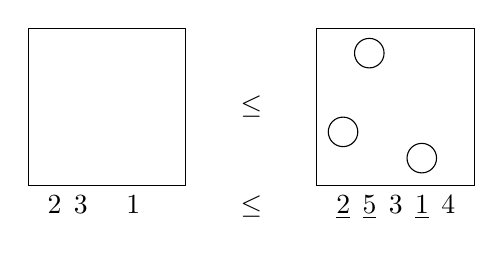
\begin{tikzpicture}[scale={1/3}, baseline=(current bounding box.center)]
		% The permutation:
		\draw (0,0) rectangle (6,6);
		\plotpartialperm{1/2,2/5,4/1};
		% Labels:
		\node at (1,0) [below] {$2$};
		\node at (2,0) [below] {$3$};
		\node at (4,0) [below] {$1$};
		
		\begin{scope}[shift={(8.5,0)}]
			\node at (0,3) {$\le$};
			\node at (0,0) [below] {$\le$};
	%			\node at (0,0) [below] {\phantom{$1$}};
		\end{scope}

		\begin{scope}[shift={(11,0)}]
			% The permutation:
			\draw (0,0) rectangle (6,6);
			\plotperm{2,5,3,1,4};
			% The containment of 231---can't use \plotpermencircle because of strange font sizes.
			\begin{scope}[xshift=-0.15pt, yshift=+1.45pt]
				\draw (1,2) circle (16pt);
				\draw (2,5) circle (16pt);
				\draw (4,1) circle (16pt);
			\end{scope}
			% Labels:
			\node at (1,0) [below] {$\underline{2}$};
			\node at (2,0) [below] {$\underline{5}$};
			\node at (3,0) [below] {$3$};
			\node at (4,0) [below] {$\underline{1}$};
			\node at (5,0) [below] {$4$};
		\end{scope}
	\end{tikzpicture}
\caption{An example of permutation containment displayed through their plots.}
\label{fig-perm-plots}
\end{figure}

Before introducing the universality problem for permutations, we give a few definitions that will be helpful throughout this chapter. Given permutations $\pi$ and $\sigma$ of respective sizes $m$ and $n$, their \emph{direct sum} is the permutation $\pi\directsum\sigma$ of size $m+n$ defined by
\[
	(\pi\directsum\sigma)(i)
	=
	\left\{\begin{array}{ll}
		\pi(i)         &\text{if $  1 \le i \le m$,}\\
		\sigma(j-m)+m  &\text{if $m+1 \le i \le m+n$.}
	\end{array}\right.
\]
Pictorially, the plot of $\pi\directsum\sigma$ consists of the plot of $\sigma$ placed above and to the right of the plot of $\pi$, as shown on the left of Figure~\ref{fig-sums}. Similarly, we define the \emph{skew sum} of $\pi$ and $\sigma$ by
\[
	(\pi\skewsum\sigma)(i)
	=
	\left\{\begin{array}{ll}
		\pi(i) + n  &\text{if $  1 \le i \le m  $,}\\
		\sigma(j-m) &\text{if $m+1 \le i \le m+n$.}
	\end{array}\right.
\]
Pictorially, the plot of $\pi\skewsum\sigma$ consists of the plot of $\sigma$ placed below and to the right of the plot of $\pi$, as shown on the right of Figure~\ref{fig-sums}. A permutation that cannot be written as a direct sum (resp. skew sum) is said to be \emph{sum-indecomposable} (resp. \emph{skew-indecomposable}.)

\begin{figure}
	\begin{tikzpicture}[scale=0.2, baseline=(current bounding box.center)]
		\node at (-4, 4.75) {$\pi\directsum\sigma = $};
		\plotpermbox{1}{1}{4}{4};
		\plotpermbox{5}{5}{8}{8};
		\node at (2.5,2.5) {$\pi$};
		\node at (6.5,6.5) {$\sigma$};

		\begin{scope}[shift={(20,0)}]
			\node at (-4, 4.75) {$\pi\skewsum\sigma = $};
			\plotpermbox{1}{5}{4}{8};
			\plotpermbox{5}{1}{8}{4};
			\node at (2.5,6.5) {$\pi$};
			\node at (6.5,2.5) {$\sigma$};
		\end{scope}
	\end{tikzpicture}
\caption{The plot of the direct sum of $\pi$ and $\sigma$ on the left and the plot of the skew sum of $\pi$ and $\sigma$ on the right.}
\label{fig-sums}
\end{figure}

As usual, we say that a permutation is $m$-universal if it contains all permutations of size $m$ as patterns. Such a permutation is sometimes called an \emph{$m$-superpattern} (for example, by B\'ona~\cite[Chapter 5, Exercises 19--22 and Problems Plus 9--12]{bona:combinatorics-o:}.) The first result about universal permutations was obtained by Simion and Schmidt in 1985~\cite[Section~5]{simion:restricted-perm:}, who computed the number of $3$-universal permutations of size $n \ge 5$ to be
\[
	n!
	- 6 C_n
	+ 5 \cdot 2^n
	+ 4 \binom{n}{2}
	- 2F_n
	- 14n
	+ 20.
\]
(Here $C_n$ denotes the $n$th Catalan number and $F_n$ denotes the $n$th \emph{combinatorial} Fibonacci number, so $F_0=F_1=1$ and $F_n=F_{n-1}+F_{n-2}$ for $n\ge 2$.) Simion and Schmidt did not use the term ``universal'' and received their formula as a corollary to a sequence of results enumerating those permutation classes where membership is defined by avoiding sets of $3$-patterns. The first to study the universal permutation problem for general $m$ was Arratia~\cite{arratia:on-the-stanley-:} in 1999.

Let $\u(m)$ denote the size of the smallest $m$-universal permutation. Arratia observed that for any permutation of size $n$ to be $m$-universal, it must have at least $m!$ length-$m$ subsequences, and thus
\[
	\binom{n}{m}
	\ge
	m!.
\]
This simple inequality, together with the inequalities $\left(\frac{ne}{m}\right)^m \ge \binom{n}{m}$ and $m! \ge \left(\frac{m}{e}\right)^m$, implies that $n \ge m^2/e^2$. This also follows from Observation~\ref{obs-alstrup-rauhe}, again using that $m! \ge \left(\frac{m}{e}\right)^m$.

Arratia also provided a simple construction of an $m$-universal permutation of size $m^2$, proving that $\u(m) = \oTheta{m^2}$. Consider the permutation whose plot consists of an $m \times m$ grid of points, with sides initially parallel to the axes, then rotated slightly clockwise. More precisely, partition the integers $1$ to $m^2$ into congruence classes modulo $m$, write each congruence class in increasing order, and then concatenate these sequences in decreasing order according to their first element. The left panel of Figure~\ref{fig-tilted-square} displays the plot of the $4$-universal permutation constructed in this manner. Arratia observed that such a permutation is $m$-universal, as the point $(i, \pi(i))$ of the pattern $\pi$ of size $m$ can simply embed into the point $i$th column (from the left) and $\pi(i)$th row (from the bottom). This kind of embedding actually allows for much more freedom in the universal permutations formed: dividing the square $(0, m^2] \times (0, m^2]$ into $m^2$ many $m \times m$ squares, this construction demonstrates that any permutation whose canonical plot places precisely $1$ point in each sqaure is $m$-universal. We exhibit another $4$-universal permutation of size $16$ that meets this criteria in the right panel of Figure~\ref{fig-tilted-square}.

\begin{figure}[ht]
\captionsetup{justification=centering}
	\begin{tikzpicture}[scale=0.25]
		\plotpermborder{4,8,12,16,3,7,11,15,2,6,10,14,1,5,9,13}

		\draw ( 4.5,0.5) -- ++(0,16);
		\draw ( 8.5,0.5) -- ++(0,16);
		\draw (12.5,0.5) -- ++(0,16);

		\draw (0.5, 4.5) -- ++(16,0);
		\draw (0.5, 8.5) -- ++(16,0);
		\draw (0.5,12.5) -- ++(16,0);

		\begin{scope}[shift={(20,0)}]
			\plotpermborder{6, 13, 9, 1, 11, 2, 5, 15, 10, 8, 4, 16, 14, 3, 12, 7}

			\draw ( 4.5,0.5) -- ++(0,16);
			\draw ( 8.5,0.5) -- ++(0,16);
			\draw (12.5,0.5) -- ++(0,16);

			\draw (0.5, 4.5) -- ++(16,0);
			\draw (0.5, 8.5) -- ++(16,0);
			\draw (0.5,12.5) -- ++(16,0);
		\end{scope}
		
	\end{tikzpicture}
\caption{The $4 \times 4$ tilted-square permutation and another $4$-universal permutation of size $16$.}
\label{fig-tilted-square}
\end{figure}

The first to improve upon these trivial bounds provided by Arratia were Eriksson, Eriksson, Linusson, and W\"{a}stlund~\cite{eriksson:dense-packing-o:}, who used probabilistic methods to construct an $m$-universal permutation of size $(2/3 + \oo{1})m^2$. The next improvement came in~\cite{miller:asymptotic-boun:}, wherein Miller proves that there is a word over the alphabet $[m+1]$ of length $(m^2 + m)/2$ that contains subsequences order-isomorphic to every permutation of size $m$. Miller noted that by ``breaking ties'' between the letters of such a word, one obtains an $m$-universal permutation of size $(m^2 + m)/2$.

\begin{theorem}[Miller~\cite{miller:asymptotic-boun:}]
	\label{thm-miller-perms}
	For all $m \ge 1$, there is a word over the alphabet $[m+1]$ of length $(m^2+m)/2$ containing subsequences order-isomorphic to every permutation of size $m$.
\end{theorem}
	
To establish this result, define the \emph{infinite zigzag word} to be the word formed by alternating between ascending \emph{runs} of the odd positive integers $1357\cdots$ and descending \emph{runs} of the even positive integers $\cdots 8642$,
\[
	(1357\cdots)\ (\cdots 8642)\ 
	(1357\cdots)\ (\cdots 8642)\ 
	(1357\cdots)\ (\cdots 8642)\ \cdots.
\]
While this object does not conform to most definitions of the word \emph{word} in combinatorics, we hope the reader forgives the slight expansion of the definition adopted here. We are interested in the leftmost embeddings of words over $\mathbb{P}$ into the infinite zigzag word.

We also need two definitions. First, given a word $p\in\mathbb{P}^\ast$, we define the word $p^{+1}\in\mathbb{P}^\ast$ to be the word formed by adding $1$ to each letter of $p$, so $p^{+1}(i)=p(i)+1$ for all indices $i$ of $p$. Next we say that the word $p\in\mathbb{P}^\ast$ has an \emph{immediate repetition} if there is an index $i$ with $p(i)=p(i+1)$, i.e., if $p$ contains a factor equal to $\ell\ell$ for some letter $\ell\in\mathbb{P}$.

\begin{proposition}[Miller~\cite{miller:asymptotic-boun:}]
	\label{prop-miller-words}
	If the word $p\in\mathbb{P}^m$ has no immediate repetitions, then either $p$ or $p^{+1}$ occurs as a subsequence of the first $m$ runs of the infinite zigzag word.
\end{proposition}

Before proving Proposition~\ref{prop-miller-words}, note that permutations do not have immediate repetitions. Thus if $\pi$ is a permutation of size $m$, Proposition~\ref{prop-miller-words} implies that either $\pi$ or $\pi^{+1}$ occurs as a subsequence in the first $m$ runs of the infinite zigzag word. Since $\pi^{+1}$ is order-isomorphic to $\pi$ and both $\pi$ and $\pi^{+1}$ are words over $[m+1]$, this implies that the restriction of the first $m$ runs of the infinite zigzag word to the alphabet $[m+1]$ contains every permutation of size $m$. For example, in the case of $m=5$ we obtain the universal word
\[
	135\ 642\ 135\ 642\ 135
\]
of length $15$ over the alphabet $[6]$.

The restriction of the infinite zigzag word described above consists of $m$ runs of average length $(m+1)/2$: if $m$ is odd, then all runs are of this length, while if $m$ is even, then half are of length $m/2$ and half are of length $(m+2)/2$. Thus Proposition~\ref{prop-miller-words} implies Theorem~\ref{thm-miller-perms}. While Proposition~\ref{prop-miller-words} does not appear explicitly in \cite{miller:asymptotic-boun:}, its proof, presented below, is adapted from Miller's proof of Theorem~\ref{thm-miller-perms}.

\newenvironment{proof-of-prop-miller-words}{%
	\medskip\noindent {\it Proof of Proposition~\ref{prop-miller-words}.\/}%
}{%
	\qed\bigskip%
}
%
\begin{proof-of-prop-miller-words}
	We define the \emph{score} of the word $p\in\mathbb{P}^\ast$, denoted by $s(p)$, as the minimum number of runs that an initial segment of the infinite zigzag word must have in order to contain $p$, minus the length of $p$. Thus our goal is to show that for every word $p\in\mathbb{P}^\ast$ without immediate repetitions, either $s(p)\le 0$ or $s(p^{+1})\le 0$. In fact, we show that for such words we have $s(p)+s(p^{+1})=1$, which implies this.

	We prove this claim by induction on the length of $p$. For the base case, we see that words consisting of a single odd letter are contained in the first run of the infinite zigzag word (thus corresponding to scores of $0$) while words consisting of a single even letter are contained in the second run (corresponding to scores of $1$). Thus for every $\ell\in\mathbb{P}^1$ we have $s(\ell)+s(\ell^{+1})=1$, as desired. Now suppose that the claim is true for all words $p\in\mathbb{P}^m$ without immediate repetitions and let $\ell\in\mathbb{P}$ denote a letter. We see that, for any $p \in \mathbb{P}^m$,
	\[
		s(p\ell)-s(p)
		=
		\left\{
		\begin{array}{cl}
			-1&	\begin{array}{l}
				\text{if $p(n)<\ell$ and both entries are odd or}\\
				\text{if $p(n)>\ell$ and both entries are even;}
				\end{array}
			\\[12pt]
			0&	\begin{array}{l}
				\text{if $p(n)$ and $\ell$ are of different parity; or}
				\end{array}
			\\[8pt]
			+1&	\begin{array}{l}
				\text{if $p(n)<\ell$ and both entries are even,}\\
				\text{if $p(n)=\ell$, or}\\
				\text{if $p(n)>\ell$ and both entries are odd.}
				\end{array}
		\end{array}
		\right.
	\]
	Because our words do not have immediate repetitions, we can ignore the possibility that $\ell=p(m)$. In the other cases, it can be seen by inspection that
	\[
		\big(  s(p\ell)-s(p)  \big)
		+
		\big(  s\!\left((p\ell)^{+1}\right) - s\!\left(p^{+1}\right)\!  \big)
		=
		0.
	\]
	By rearranging these terms, we see that
	\[
		s(p\ell) + s\!\left((p\ell)^{+1}\right)
		=
		s(p)+s\!\left(p^{+1}\right).
	\]
	Since $s(p)+s\!\left(p^{+1}\right)=1$ by induction, this completes the proof of the inductive claim, and thus also of the proposition.
\end{proof-of-prop-miller-words}

Here, we give a new improvement to Miller's upper bound. In order to do so, we further restrict the infinite zigzag word, and then break ties between its letters to obtain a specific permutation $\zeta_m$. To this end, we define the word $z_m$ to be the restriction of the first $m$ runs of the infinite zigzag word to the alphabet $[m]$. When $m$ is even, each run of $z_m$ has length $m/2$. When $m$ is odd, $z_m$ consists of $(m+1)/2$ ascending odd runs, each of length $(m+1)/2$, and $(m-1)/2$ descending even runs, each of length $(m-1)/2$. Thus we have
\[
	\size{z_m}
	=
	\left\{
	\begin{array}{cl}
		\displaystyle\frac{m^2}{2}  &\text{if $m$ is even,}\\[12pt]
		\displaystyle\frac{m^2+1}{2}&\text{if $m$ is odd.}
	\end{array}
	\right.
\]

As one additional definition, we say that a word $u$ is \emph{order-homomorphic} to another word $v$ of the same length if for all indices $i$ and $j$, we have
\[
	u(i) > u(j)
	\implies
	v(i) > v(j).
\]
Next, we choose a specific permutation, $\zeta_m$, such that $z_m$ is order-homomorphic to $\zeta_m$. In constructing $\zeta_m$, we have the freedom to break ties between equal letters of $z_m$. That is to say, if $z_m(i)=z_m(j)$ for $i\neq j$, then in constructing $\zeta_m$ we may choose whether $\zeta_m(i)<\zeta_m(j)$ or $\zeta_m(i)>\zeta_m(j)$ arbitrarily without affecting any other pair of comparisons and thus without losing any occurrences of permutations. We choose to break these ties by replacing all instances of a given letter $k\in[m]$ in $z_m$ by a decreasing subsequence in $\zeta_m$. Thus for indices $i<j$, we have
\[
	z_m(i)=z_m(j)
	\implies
	\zeta_m(i)>\zeta_m(j).
\]
This choice uniquely determines $\zeta_m$ (up to order-isomorphism), as all comparisons between its letters are determined either in $z_m$, if the corresponding letters of $z_m$ differ, or by the rule above, if the corresponding letters of $z_m$ are the same. Figure~\ref{fig-z5-zeta5} shows the plots of $z_5$ and $\zeta_5$, where the \emph{plot} of a word $w$ over $\mathbb{P}$ is the set $\{(i,w(i))\}$ of points in the plane.

\begin{figure}[ht]
\captionsetup{justification=centering}
	\begin{footnotesize}
		\begin{tabular}{ccc}
			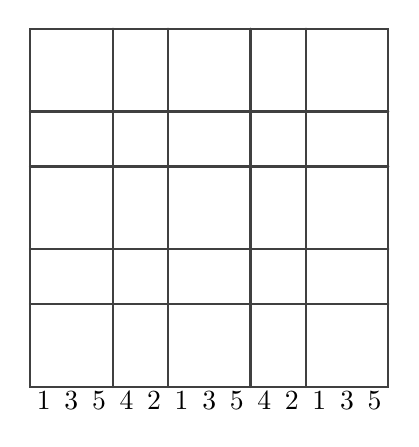
\begin{tikzpicture}[scale=0.35, baseline=(current bounding box.south)]
				\foreach \y/\val [count = \x] in {1/2, 3/7, 5/12, 4/9.5, 2/4.5, 1/2, 3/7, 5/12, 4/9.5, 2/4.5, 1/2, 3/7, 5/12} {
					\absdot{(\x,\val)}
					\node at (\x, 0) {\y};
					}
				\draw[darkgray, thick, line cap=round] (0.5,0.5) rectangle (13.5,13.5);
				\foreach \y in {3,5,8,10} {
					\draw[darkgray, thick, line cap=round] (0.5, \y+0.5) -- (13.5, \y+0.5);
					\draw[darkgray, thick, line cap=round] (\y+0.5, 0.5) -- (\y+0.5, 13.5);
				}
			\end{tikzpicture}
			&\quad\quad&
			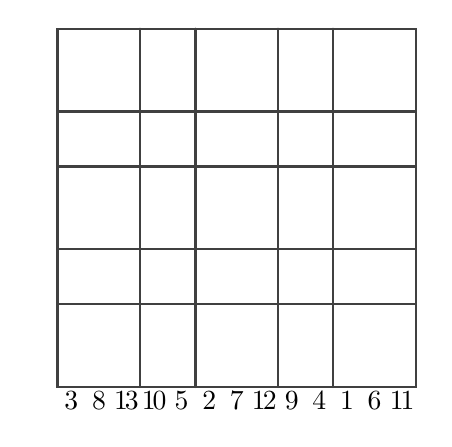
\begin{tikzpicture}[scale=0.35, baseline=(current bounding box.south)]
				\plotperm{3,8,13,10,5,2,7,12,9,4,1,6,11}
				% The labels
				\node at (1,0) {3};
				\node at (2,0) {8};
				\node at (3,0) {1\!\!\:3};
				\node at (4,0) {1\!\!\:0};
				\node at (5,0) {5};
				\node at (6,0) {2};
				\node at (7,0) {7};
				\node at (8,0) {1\!\!\:2};
				\node at (9,0) {9};
				\node at (10,0) {4};
				\node at (11,0) {1};
				\node at (12,0) {6};
				\node at (13,0) {1\!\!\:1};
				\draw[darkgray, thick, line cap=round] (0.5,0.5) rectangle ++(13,13);
				\foreach \y in {3,5,8,10} {
					\draw[darkgray, thick, line cap=round] (0.5, \y+0.5) -- ++(13, 0);
					\draw[darkgray, thick, line cap=round] (\y+0.5, 0.5) -- ++(0, 13);
				}
				\node at (0,0) {\phantom{1}};
			\end{tikzpicture}
		\end{tabular}
	\end{footnotesize}
\caption{On the left, the further restriction we define of the infinite zigzag word, $z_5$. On the right, the normalized permutation formed by breaking ties, $\zeta_5$.}
\label{fig-z5-zeta5}
\end{figure}

In the following sequence of results, we show that $\zeta_m$ is \emph{almost} universal. In fact, we show that $\zeta_m$ fails to be universal only for even $m$, and in that case, the only missing permutation is the decreasing permutation $m\cdots 21$. The first of these results, Proposition~\ref{prop-distant-inv-desc}, covers almost all permutations. (In fact, Proposition~\ref{prop-distant-inv-desc-layered} shows that Proposition~\ref{prop-distant-inv-desc} handles all but $2^{m-1}$ permutations of size $m$.)

We say that two entries $\pi(j)$ and $\pi(k)$ form an \emph{inverse-descent} if $j<k$ and $\pi(j)=\pi(k)+1$. (As the name is meant to indicate, if a pair of entries forms an inverse-descent in $\pi$, then the corresponding entries of $\pi^{-1}$ form a descent.) If $\pi(j)$ and $\pi(k)$ form an inverse-descent and they are not adjacent in $\pi$ (so $k\ge j+2$), then we say that they form a \emph{distant} inverse-descent.

\begin{proposition}
	\label{prop-distant-inv-desc}
	If the permutation $\pi$ of size $m$ has a distant inverse-descent, then $\zeta_m$ contains a subsequence order-isomorphic to $\pi$.
\end{proposition}
\begin{proof}
	Suppose that the entries $\pi(a)$ and $\pi(b)$ form a distant inverse-descent in $\pi$, meaning that $\pi(a)=\pi(b)+1$ and $b\ge a+2$. We define the word $p\in [m-1]^m$ by
	\[
		p(i)
		=
		\left\{\begin{array}{ll}
			\pi(i)   &\text{if $\pi(i)\le\pi(b)$,}\\
			\pi(i)-1 &\text{if $\pi(i)\ge\pi(a)=\pi(b)+1$.}
		\end{array}\right.
	\]

	The word $p$ has two occurrences of the letter $\pi(b)$, but because $\pi(a)$ and $\pi(b)$ form a distant inverse-descent, these two occurrences of $\pi(b)$ in $p$ do not constitute an immediate repetition. Thus Proposition~\ref{prop-miller-words} shows that either $p$ or $p^{+1}$ occurs as a subsequence in the first $n$ runs of the infinite zigzag word. As $p$ and $p^{+1}$ are both words over $[m]$, whichever of these words occurs in the first $n$ runs of the infinite zigzag word  also occurs as a subsequence of $z_m$. Suppose that this subsequence occurs in the indices $1\le i_1<i_2<\cdots<i_m\le \size{z_m}$, so $z_m(i_1)z_m(i_2)\cdots z_m(i_m)$ is equal to either $p$ or $p^{+1}$, and thus for $j,k \in [m]$ we have
	\[
		z_m(i_j) > z_m(i_k)
		\iff 
		p(j) > p(k).
	\]
	Because $z_m$ is order-homomorphic to $\zeta_m$, this implies that for all pairs of indices $j,k\in[m]$ except the pair $\{a,b\}$, we have
	\[
		\zeta_m(i_j) > \zeta_m(i_k)
		\iff 
		p(j) > p(k)
		\iff 
		\pi(j) > \pi(k).
	\]
	Furthermore, since $p(a)=p(b)$, we have $z_m(a)=z_m(b)$, and so by our construction of $\zeta_m$ it follows that $\zeta_m(a)>\zeta_m(b)$, while we know that $\pi(a)>\pi(b)$ because those entries form an inverse-descent. This verifies that $\zeta_m(i_1)\zeta_m(i_2)\cdots \zeta_m(i_m)$ is order-isomorphic to $\pi$, completing the proof.
\end{proof}

\begin{figure}[ht]
	\captionsetup{justification=centering}
		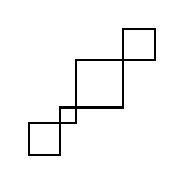
\begin{tikzpicture}[scale=0.2, baseline=(current bounding box.center)]
			\draw[thick] (0.5, 0.5)
				rectangle ++(2,2)
				rectangle ++(1,1)
				rectangle ++(3,3)
				rectangle ++(2,2);
			% The permutation:
			\begin{scope}[shift={(0,-1pt)}]
				\plotperm{2,1,3,6,5,4,8,7};
			\end{scope}
		\end{tikzpicture}
	\caption{The plot of the layered permutation $21\ 3\ 654\ 87$ with layer lengths $2$, $1$, $3$, $2$.}
	\label{fig-layered}
\end{figure}

To describe the permutations that Proposition~\ref{prop-distant-inv-desc} does not apply to, we need the notion of a layered permutation. A permutation is said to be \emph{layered} if it can be expressed as a sum of decreasing permutations, and in this case, these decreasing permutations are themselves called the \emph{layers}. An example of a layered permutation is shown in Figure~\ref{fig-layered}.

\begin{proposition}
	\label{prop-distant-inv-desc-layered}
	The permutation $\pi$ is layered if and only if it does not have a distant inverse-descent.
\end{proposition}
\begin{proof}
	One direction is completely trivial: if $\pi$ is layered then all of its inverse-descents are between consecutive entries, so it does not have a distant inverse-descent. For the other direction, we use induction on the size of $\pi$. The empty permutation is layered, so the base case holds. If $\pi$ is a nonempty permutation without distant inverse-descents, then it must begin with the entries $\pi(1)$, $\pi(1)-1$, $\dots$, $2$, $1$ in that order. This means that $\pi=\delta\directsum\sigma$ where $\delta$ is a nonempty decreasing permutation and $\sigma$ is a permutation smaller than $\pi$ that also does not have any distant inverse-descents. By induction, $\sigma$ is layered, and thus $\pi$ is as well, completing the proof.
\end{proof}

Having characterized the permutations to which Proposition~\ref{prop-distant-inv-desc} does not apply, we now show that almost all of them are nevertheless contained in $\zeta_m$.

\begin{proposition}
	\label{prop-layered-zeta}
	If the permutation $\pi$ of size $n$ is layered and not a decreasing permutation of even size, then $\zeta_m$ contains a subsequence order-isomorphic to $\pi$.
\end{proposition}
\begin{proof}
	Let $\pi$ denote an arbitrary layered permutation of size $n$. To prove the result, we compute the score of $\pi$ as in the proof of Proposition~\ref{prop-miller-words}, show that this score can only take on the values $0$ or $\pm 1$, and then describe an alternative embedding of $\pi$ in $\zeta_m$ in the case where the score of $\pi$ is $1$, except when $\pi$ is a decreasing permutation of even size.

	Recall that the score of any word $\pi$, $s(\pi)$, is defined as the number of initial runs of the infinite zigzag word necessary to contain $\pi$ minus the size of $\pi$. As observed in the proof of Proposition~\ref{prop-miller-words}, the score of a word does not change upon reading a letter of opposite parity. This implies that, while reading a layered permutation, the score changes only when transitioning from one layer to the next, and thus we compute the score of $\pi$ layer-by-layer.

	\renewcommand{\OE}{\textsf{odd}\text{--}\textsf{even}}
	\newcommand{\OO}{\textsf{odd}\text{--}\textsf{odd}}
	\newcommand{\EE}{\textsf{even}\text{--}\textsf{even}}
	\newcommand{\EO}{\textsf{even}\text{--}\textsf{odd}}

	\begin{figure}[ht]
	\captionsetup{justification=centering}
		\begin{footnotesize}
			\begin{tikzpicture}[
				scale=1, 
				xscale=3, 
				node style/.style={thick, draw, ellipse, minimum width=68pt, minimum height = 16.66666pt, align=center}
			]

				\draw (-1, 0) node[node style] (oe) {$\OE$};
				\draw ( 0,-1) node[node style] (ee) {$\EE$};
				\draw ( 0, 1) node[node style] (oo) {$\OO$};
				\draw ( 1, 0) node[node style] (eo) {$\EO$};
				
				\draw [->] (0,-{1.6}) to (0,-{1.333333});
				
				% \draw [->] (eo) to (oo);
				\draw [-] (+0.9, +0.4) to (+0.9,+0.8);
				\draw [domain=0:90] plot ({+0.833333+0.066667*cos(\x)}, {+0.8+0.2*sin(\x)});
				\draw [->] (+0.833333,+1.0) to (+0.425, +1.0);
				\node at (0.8,0.8) {$-1$};
				
				% \draw [->] (oo) to (oe);
				\draw [-] (-0.425, 1.0) to (-0.833333,1.0);
				\draw [domain=90:180] plot ({-0.833333+0.066667*cos(\x)}, {0.8+0.2*sin(\x)});
				\draw [->] (-0.9,0.8) to (-0.9, 0.4);
				\node at (-0.8,0.8) {$-1$};
				
				% \draw [->] (oe) to (ee);
				\draw [-] (-0.9, -0.4) to (-0.9,-0.8);
				\draw [domain=180:270] plot ({-0.833333+0.066667*cos(\x)}, {-0.8+0.2*sin(\x)});
				\draw [->] (-0.833333,-1.0) to (-0.5, -1.0);
				\node at (-0.8,-0.8) {$+1$};
				
				% \draw [->] (ee) to (eo);
				\draw [-] (+0.5, -1.0) to (+0.833333,-1.0);
				\draw [domain=270:360] plot ({+0.833333+0.066667*cos(\x)}, {-0.8+0.2*sin(\x)});
				\draw [->] (+0.9,-0.8) to (+0.9, -0.4);
				\node at (+0.8,-0.8) {$+1$};
				
				% \draw [->] (oe) to (oe);
				\newcommand\hmargin{0.0666667}
				\newcommand\vmargin{0.2}
				\newcommand\leftloopleft{-1.45}
				\newcommand\leftloopright{-1.166667}
				\newcommand\loopupper{0.45}
				\newcommand\looplower{-\loopupper}
				
				\draw [-] (\leftloopright+\hmargin, 0.4) to (\leftloopright+\hmargin,\loopupper);
				\draw [domain=  0: 90] plot ({\leftloopright+\hmargin*cos(\x)}, {\loopupper+\vmargin*sin(\x)}); % NE corner
				\draw [-] (\leftloopright, \loopupper+\vmargin) to (\leftloopleft,\loopupper+\vmargin);
				\draw [domain= 90:180] plot ({\leftloopleft+\hmargin*cos(\x)}, {\loopupper+\vmargin*sin(\x)}); % NW corner
				\draw [-] (\leftloopleft-\hmargin,\loopupper) to (\leftloopleft-\hmargin, \looplower);
				\draw [domain=180:270] plot ({\leftloopleft+\hmargin*cos(\x)}, {\looplower+\vmargin*sin(\x)}); % SW corner
				\draw [-] (\leftloopright, \looplower-\vmargin) to (\leftloopleft,\looplower-\vmargin);
				\draw [domain=270:360] plot ({\leftloopright+\hmargin*cos(\x)}, {\looplower+\vmargin*sin(\x)}); % SE corner
				\draw [->] (\leftloopright+\hmargin,\looplower) to (\leftloopright+\hmargin, -0.4);
				\node at (\leftloopleft,\loopupper) {$0$};
				
				% \draw [->] (eo) to (eo);
				\newcommand\rightloopright{-\leftloopleft}
				\newcommand\rightloopleft{-\leftloopright}

				\draw [-] (\rightloopleft-\hmargin,-0.4) to (\rightloopleft-\hmargin, \looplower);
				\draw [domain=180:270] plot ({\rightloopleft+\hmargin*cos(\x)}, {\looplower+\vmargin*sin(\x)}); % NE corner
				\draw [-] (\rightloopright, \looplower-\vmargin) to (\rightloopleft,\looplower-\vmargin);
				\draw [domain=270:360] plot ({\rightloopright+\hmargin*cos(\x)}, {\looplower+\vmargin*sin(\x)}); % NW corner
				\draw [-] (\rightloopright+\hmargin,\looplower) to (\rightloopright+\hmargin, \loopupper);
				\draw [domain=  0: 90] plot ({\rightloopright+\hmargin*cos(\x)}, {\loopupper+\vmargin*sin(\x)}); % SW corner
				\draw [-] (\rightloopright, \loopupper+\vmargin) to (\rightloopleft,\loopupper+\vmargin);
				\draw [domain= 90:180] plot ({\rightloopleft+\hmargin*cos(\x)}, {\loopupper+\vmargin*sin(\x)}); % SE corner
				\draw [->] (\rightloopleft-\hmargin, \loopupper) to (\rightloopleft-\hmargin,0.4);
				\node at (\rightloopright,\looplower) {\footnotesize$0$};


				\node at (-0.8,-0.8) {$+1$};

				% \draw [->] (oo) to (ee);
				\draw [->] (-0.1,0.575) to (-0.1,-0.625);
				\node at (-0.15,0) {$0$};
				
				% \draw [->] (ee) to (oo);
				\draw [->] (+0.1,-0.625) to (+0.1,+0.575);
				\node at (+0.15,0) {$0$};
				
			\end{tikzpicture}
		\end{footnotesize}
		\caption{A directed graph describing the scoring of a layered permutation.}
		\label{fig-layered-zeta-automaton}
	\end{figure}

	The change in score when moving from one layer of $\pi$ to the next is determined by the parity of the last entry of the layer we are leaving and the first entry of the layer we are entering. Specifically, the score changes by $-1$ if both of these entries are odd and $+1$ if both are even. This shows that in order to compute the score of the layered permutation $\pi$, we simply need to know the parities of the first and last entries of each of its layers. This information is represented by the labels of the nodes of the directed graph shown in Figure~\ref{fig-layered-zeta-automaton}.

	Moreover, not all transitions between these nodes are possible, because the last entry of a layer is precisely $1$ greater than the first entry of the preceding layer. This is why there are only eight edges shown in Figure~\ref{fig-layered-zeta-automaton}. In this figure, each of those edges is labeled by the change in the score function. Note that the first layer must end with $1$ (an odd entry), and its first entry must be either odd (for a score of $0$) or even (for a score of $1$); this is equivalent to starting our walk on the graph in Figure~\ref{fig-layered-zeta-automaton} at the node labeled $(\EE)$ before any layers are read.

	From this graphical interpretation of the scoring process, it is apparent that the score of a layered permutation can take on only three values: $-1$ if it ends at the node $(\OE)$; $0$ if it ends at either node $(\EE)$ or $(\OO)$; or $1$ if it ends at the node $(\EO)$. Except in this final case, we are done.

	Now suppose that we are in the final case, so the ultimate layer of $\pi$ is of $(\EO)$ type. The first entry of this layer is the greatest entry of $\pi$, so we know that $\pi$ has even size. If $\pi$ were a decreasing permutation then there would be nothing to prove (as we have not claimed anything in this case), so let us further suppose that $\pi$ is not a decreasing permutation, and thus that $\pi$ has at least two layers. We further divide this case into two cases. In both cases, as in the proof of Proposition~\ref{prop-distant-inv-desc}, we construct a word $p\in[m-1]^m$ such that if $z_m$ contains $p$, then $\zeta_m$ contains $\pi$.

	First, suppose that the penultimate layer of $\pi$ is of $(\EO)$ type and that this layer begins with the entry $\pi(b)$. This implies that the penultimate layer of $\pi$ has at least two entries (because its first and last entries have different parities). In this case, we define $p$ by
	\[
		p(i)
		=
		\left\{\begin{array}{ll}
			\pi(i)&\text{if $\pi(i)<\pi(b)$,}\\
			\pi(i)-1&\text{if $\pi(i)\ge\pi(b)$.}
		\end{array}\right.
	\]
	In other words, to form $p$ from $\pi$ we decrement the first entry of the penultimate layer and all entries of the ultimate layer. Because the penultimate layer of $\pi$ has at least two entries, performing this operation creates an immediate repetition (of the entry $\pi(b)-1$) at the beginning of this layer. For example, if $\pi=21\ 6543\ 87$ then $\pi(b)=6$ and we decrement the $6$, $8$, and $7$ to obtain the word $p=21\ 5543\ 76$.

	As with our previous constructions, if $z_m$ contains an occurrence of $p$, then $\zeta_m$ will contain a copy of $\pi$. We establish that $z_m$ contains $p$ by showing that $s(p)=0$, which requires a further bifurcation into subcases. In both subcases, the scoring of $p$ is computed by considering its score in the antepenultimate layer (the layer immediately before the penultimate layer), the score change when reading the newly decremented first entry of the penultimate layer, the score penalty of $+1$ because $p$ contains an immediate repetition (namely, $\pi(b)-1$ occurs twice in a row), and finally the score change between the penultimate and ultimate layers. We label these cases by the final three nodes of the directed graph from Figure~\ref{fig-layered-zeta-automaton} visited while computing the score of $\pi$.
	\begin{itemize}
		\item The final three layers are of type $(\EE)(\EO)(\EO)$. Note that this case includes the possibility that $\pi$ has only two layers. If $p$ has an antepenultimate layer, then the score while reading that layer is $0$ and the ascent between its last entry and the newly decremented first entry of the penultimate layer is of different parity (even to odd), contributing $0$ to the score. If $p$ does not have an antepenultimate layer, then $p$ begins with the newly decremented first entry of its penultimate layer, which contributes $0$ to the score. In either case, the score of $p$ is $0$ upon reading the first entry of the penultimate layer. The immediate repetition in the penultimate layer contributes $+1$ to the score, while the ascent between the last entry of the penultimate layer and the newly decremented first entry of the ultimate layer is odd and thus contributes $-1$, so $s(p) = 0$.
		\item The final three layers are of type $(\EO)(\EO)(\EO)$. The score while reading the antepenultimate layer is $+1$. The ascent between the last entry of the antepenultimate layer and the newly decremented first entry of the penultimate layer is odd, so it contributes $-1$ to the score, the immediate repetition in the penultimate layer contributes $+1$, and the ascent between the last entry of the penultimate layer and the newly decremented first entry of the ultimate layer is odd and thus contributes $-1$, so $s(p) = 0$.
	\end{itemize}

	It remains to treat the case where the penultimate layer is of $(\EE)$ type. Note that this case includes the possibility that the penultimate layer consists of a single entry. Suppose that the penultimate layer ends with the entry $\pi(a)$. We define $p$ by
	\[
		p(i)
		=
		\left\{\begin{array}{ll}
			\pi(i)   &\text{if $\pi(i)<\pi(a)$ or $\pi(i)=m$,}\\
			\pi(i)+1 &\text{if $\pi(i)\ge\pi(a)$ and $\pi(i)\neq m$.}
		\end{array}\right.
	\]
	Thus in forming $p$ from $\pi$ we increment all entries of the penultimate layer and all but the first entry of the ultimate layer. For example, if $\pi=21\ 3\ 654\ 87$, then we increment the $6$, $5$, $4$, and $7$ to obtain the word $p=21\ 3\ 765\ 88$.

	As before, if $z_m$ contains an occurrence of $p$ then $\zeta_m$ will contain a copy of $\pi$. Thus we need only show that $s(p)=0$, which we do, as in the previous case, by considering the scoring of the final three layers. As in that case, we identify two subcases.
	\begin{itemize}
		\item The final three layers are of type $(\OE)(\EE)(\EO)$. The score while reading the antepenultimate layer is $-1$. The ascent between the last entry of the antepenultimate layer and the newly incremented first entry of the penultimate layer is of different parity (even to odd) and thus contributes $0$ to the score. The ascent between the newly incremented last entry of the penultimate and the first entry of the ultimate layer (which is $m$) is of different parity (odd to even) and thus contributes $0$ to the score. Finally, the immediate repetition at the beginning of the ultimate layer (the two entries equal to $m$) contributes $+1$ to the score, so $s(p)=0$.
		\item The final three layers are of type $(\OO)(\EE)(\EO)$. The score while reading the antepenultimate layer is $0$. The ascent between the last entry of the antepenultimate layer and the newly incremented first entry of the penultimate layer contributes $-1$ to the score (as both entries are now odd). The ascent between the newly incremented last entry of the penultimate layer and the first entry of the ultimate layer (which is $n$) is of different parity (odd to even) and thus contributes $0$ to the score. Finally, the immediate repetition at the beginning of the ultimate layer contributes $+1$ to the score, so $s(p)=0$.
	\end{itemize}

	As we have considered all of the cases, the proof is complete.
\end{proof}

It remains only to conclude. The size of $\zeta_m$ is $(m^2+1)/2$ when $m$ is odd and $m^2/2$ when $m$ is even. When $m$ is odd, we have established that $\zeta_m$ is $m$-universal. However, Proposition~\ref{prop-layered-zeta} shows that $\zeta_m$ need not be universal when $m$ is even. (Indeed, it can be checked that $\zeta_m$ is \emph{not} $m$-universal when $m$ is even.) However, in this case, we know that $\zeta_m$ contains the decreasing permutation $(m-1)\cdots 21$ (for instance because it contains the permutation $(m-1)\cdots 21\oplus 1$). Thus we obtain an $m$-universal permutation by prepending a new maximum entry to $\zeta_m$, giving us the following bound.

\begin{theorem}[Engen and Vatter~\cite{engen:containing-all-:}]
\label{thm-perm-universal}
There is an $m$-universal permutation of size $\ceil{(m^2+1)/2}$.
\end{theorem}

A computer search reveals that the bound in Theorem~\ref{thm-perm-universal} is best-possible for $m \le 5$. Alas, for $m=6$ the $6$-universal permutation of Theorem~\ref{thm-perm-universal}'s construction has size $19$, but Arnar Arnarson [private communication] has found that the permutation
\[
	6\ 14\ 10\ 2\ 13\ 17\ 5\ 8\ 3\ 12\ 9\ 16\ 1\ 7\ 11\ 4\ 15
\]
of size $17$ is $6$-universal, and computations have shown that no smaller permutation suffices.

Arratia~\cite[Conjecture 2]{arratia:on-the-stanley-:} conjectured that the size of the smallest $m$-universal permutations is asymptotic to $m^2/e^2$. In~\cite{chroman:lower-bounds:}, Chroman, Kwan, and Singhal prove that any $m$-universal permutation must have size at least $(1.000076/e^2)m^2$ asymptotically, refuting Arratia's conjecture. In~\cite{eriksson:dense-packing-o:}, Eriksson, Eriksson, Linusson, and W\"{a}stlund conjecture that the smallest $m$-universal permutations have size asymptotic to $m^2/2$, and in~\cite{arratia:on-the-stanley-:}, Arratia presents Alon's conjecture that, asymptotically, most permutations of size $m^2/4$ are $m$-universal.

%%%%%%%%%%%%%%%%%%%%%%%%%%%%%%%%%%%%%%%%%%%%%%%%%%%%%%%%%%%%%%%%
\section{Proper Permutation Classes}
\label{sec-perm-proper}
%%%%%%%%%%%%%%%%%%%%%%%%%%%%%%%%%%%%%%%%%%%%%%%%%%%%%%%%%%%%%%%%

In this section, we consider the problem of universality for proper permutation classes. For reference, some known or computed values of minimum sizes for universal permutations for various classes are presented in Appendix~\ref{appendix-permutations}. Every class may be described as the set of permutations that avoid each element of a set of permutations, and the minimal such set is called the \emph{basis} of the class. If $\P$ is the set of permutations that avoid the set of permutations $S$, then we write $\P = \Av(S)$.

The pattern containment order is closely related to the induced subgraph order, a connection that frequently proves useful. If $\pi$ is a permutation of size $n$, define the \emph{inversion graph} of $\pi$, denoted $\g(\pi)$, to be the graph with vertex set $[n]$ and edges $i \sim j$ if and only if $i < j$ and $\pi(i) > \pi(j)$. Then, if $\pi$ contains $\tau$ as a pattern, then $\g(\pi)$ contains $\g(\tau)$ as an induced subgraph.

For any collection of permutations $\P$, let $\g(\P) = \{\g(\pi) \st \pi \in \P\}$. Suppose that $\G$ is a class of graphs with $\G = \g(\P)$ for some permutation class $\P$. If the permutation $\pi$ is $\P_m$-universal, then $\g(\pi)$ is $\G(\P)_m$-universal. Moreover, if $\pi$ is a proper $\P_m$-universal permutation, then $\g(\pi)$ lies in $\G$, so $\g(\pi)$ is a proper $\G_m$-universal graph. This shows that $\u_\G^p(m) \le \u_\P^p(m)$, giving us the following rhombus of inequalities.

\begin{center}
\begin{tabular}{CCC}
	\u_{\G}(m) & \le & \u_{\G}^{p}(m) \\
	  \rotle   &     &     \rotle     \\
	\u_{\P}(m) & \le & \u_{\P}^{p}(m)
\end{tabular}
\end{center}

%%%%%%%%%%%%%%%%%%%%%%%%%%%%%%%%%%%%%%%%%%%%%%%%%%%%%%%%%%%%%%%%
\subsection{Layered Permutations}
\label{sec-perm-layered}
%%%%%%%%%%%%%%%%%%%%%%%%%%%%%%%%%%%%%%%%%%%%%%%%%%%%%%%%%%%%%%%%

Recall that a permutation is layered if it is the direct sum of decreasing permutations. Equivalently, a permutation is layered if it avoid the patterns $231$ and $312$. Let $\Lay = \Av(231,312)$ denote the class of layered permutations. Proposition~\ref{prop-clusterize} shows that any graph may be transformed into a cluster graph of the same size that contains each cluster graph that the original graph contained. Similarly, the following proposition, which appears in~\cite{albert:universal-layer:}, shows that any permutation may be transformed into a layered permutation of the same size while retaining each of its layered containments.

\begin{proposition}[Albert, Engen, Pantone, and Vatter~\cite{albert:universal-layer:}]
\label{prop-layerize}
	Given any permutation $\pi$ of size $n$, there is a layered permutation of size $n$ that contains every layered permutation contained in $\pi$.
\end{proposition}
\begin{proof}
	We prove the claim by induction on $n$. Note that the base case is trivial, and let $\pi$ be a permutation of size $n \ge 1$. Let $D$ denote a decreasing subsequence of $\pi$ of maximum possible size. Because $D$ is a maximal decreasing subsequence, every entry of $\pi$ that is not in $D$ must either lie to the southwest of an entry of $D$ or to the northeast of such an entry, but not both. Let $D^-$ denote the set of entries that lie to the southwest of an entry of $D$ and let $D^+$ denote the set of entries that lie to the northeast of such an entry, so that $D$, $D^-$, and $D^+$ together constitute a partition of the entries of $\pi$. An example of this decomposition is shown on the leftmost panel of Figure~\ref{fig-layerization}.

	Define $\pi^-$ (resp., $\pi^+$) to be the permutation in the same relative order as the entries of $D^-$ (resp., $D^+$). Let $\delta$ be the decreasing permutation of size $\size{D}$, and define $\pi^\ast = \pi^-\directsum\delta\directsum\pi^+$. Thus, in some sense, $\pi^\ast$ is a ``straightened-out'' version of $\pi$, and an example is shown in the central panel of Figure~\ref{fig-layerization}.

	\begin{figure}[h]
	\captionsetup{justification=centering}
		\begin{center}
			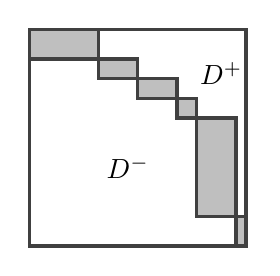
\begin{tikzpicture}[scale=0.25, baseline=(current bounding box.center)]
				\draw [darkgray, very thick, fill=lightgray] (0.5,11.5) rectangle (4,10);
				\draw [darkgray, very thick, fill=lightgray] (4,10) rectangle (6,9);
				\draw [darkgray, very thick, fill=lightgray] (6,9) rectangle (8,8);
				\draw [darkgray, very thick, fill=lightgray] (8,8) rectangle (9,7);
				\draw [darkgray, very thick, fill=lightgray] (9,7) rectangle (11,2);
				\draw [darkgray, very thick, fill=lightgray] (11,2) rectangle (11.5,0.5);
				\plotperm{3, 5, 4, 10, 1, 9, 6, 8, 7, 11, 2};
				\draw [darkgray, very thick] (0.5,0.5) rectangle (11.5,11.5);
				\node at (5.5,4.5) {$D^-$};
				\node at (10.25,9.25) {$D^+$};
			\end{tikzpicture}
			\quad\quad\quad
			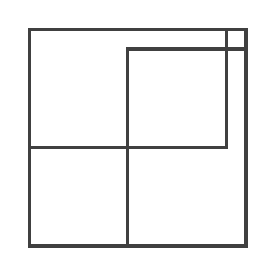
\begin{tikzpicture}[scale=0.25, baseline=(current bounding box.center)]
				\plotperm{2,4,3,5,1,10,9,8,7,6,11};
				\draw [darkgray, very thick] (0.5,0.5) rectangle (11.5,11.5);
				\draw [darkgray, very thick] (0.5,0.5) rectangle (5.5,5.5);
				\draw [darkgray, very thick] (5.5,5.5) rectangle (10.5,10.5);
				\draw [darkgray, very thick] (10.5,10.5) rectangle (11.5,11.5);
			\end{tikzpicture}
			\quad\quad\quad
			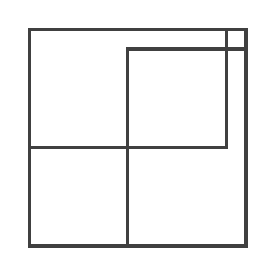
\begin{tikzpicture}[scale=0.25, baseline=(current bounding box.center)]
				\plotperm{1,4,3,2,5,10,9,8,7,6,11};
				\draw [darkgray, very thick] (0.5,0.5) rectangle ++(11,11);
				\draw [darkgray, very thick] (0.5,0.5) %
					rectangle ++(5,5) % 
					rectangle ++(5,5) %
					rectangle ++(1,1);
			\end{tikzpicture}
		\end{center}
	\caption{The steps in the proof of Proposition~\ref{prop-layerize}. From left to right, the drawings show an example of $\pi$, of $\pi^\ast$, and of the layered permutation $\tau^- \directsum \delta \directsum \tau^+$.}
	\label{fig-layerization}
	\end{figure}

	We claim that every layered permutation contained in $\pi$ is also contained in $\pi^\ast$. Suppose $\lambda=\lambda_{1}\directsum\cdots\directsum\lambda_\ell$ is a layered permutation contained in $\pi$, where each $\lambda_{i}$ is a decreasing permutation, and fix an embedding of $\lambda$ into $\pi$. Choose $j$ maximally so that in this embedding of $\lambda$ into $\pi$, the layers $\lambda_{1}\directsum\cdots\directsum\lambda_{j-1}$ are embedded entirely using entries in $D^-$. It follows that the entries of $\lambda_{j+1}\directsum\cdots\directsum\lambda_\ell$ are embedded entirely using entries of $D^+$. Since $\lambda_j$ certainly embeds into $D$ and consequently into $\delta$, we have that $\lambda \le \pi^\ast$.

	Finally, by induction we see that there are layered permutations $\mu^-$ and $\mu^+$ that contain all of the layered permutations contained in $\pi^-$ and $\pi^+$, respectively. It follows that $\mu^- \directsum \delta \directsum \mu^+$ is layered and contains all of the layered permutations contained in $\pi^\ast$, which in turn contains all of the layered permutations contained in $\pi$, proving the proposition. An example of this final construction is shown in the rightmost panel of Figure~\ref{fig-layerization}.
\end{proof}

In particular, any $\Lay_m$-universal permutation may be transformed into a layered permutation of the same size that is still $\Lay_m$-universal, affirming a conjecture of Gray~\cite{gray:bounds-on-super:}. Thus, among the smallest $\Lay_m$-universal permutations there are proper $\Lay_m$-universal permutations, establishing following corollary, which appears in~\cite{albert:universal-layer:}.
\begin{corollary}[Albert, Engen, Pantone, and Vatter~\cite{albert:universal-layer:}]
	For all integers $m \ge 0$, the smallest proper $\Lay_m$-universal permutations are also smallest $\Lay_m$-universal permutations.
\end{corollary}

We note that if $\lambda$ and $\mu$ are layered permutations with layer lengths $\lambda_1, \cdots, \lambda_m$ and $\mu_1, \cdots, \mu_n$ respectively, then we have $\lambda \le \mu$ if and only if there are indices $i_1 < i_2 < \cdots < i_m$ so that $\lambda_{j} \le \mu_{i_j}$ for all $j$. Therefore the poset of layered permutations is isomorphic to the poset of compositions under the generalized subword order discussed in Chapter~\ref{chap-compositions}. As in any question of universality for classes of layered permutations we may assume that the containing permutation is layered, we may reduce each such question to the corresponding question of universality for composition classes. Theorem~\ref{thm-comp-universal}, adapted from~\cite{albert:universal-layer:}, gives a precise formula for the size of the smallest $m$-universal compositions, and thus a formula for the size of the smallest $\Lay_m$-universal permutations.
\begin{corollary}[Albert, Engen, Pantone, and Vatter~\cite{albert:universal-layer:}]
\label{cor-perm-layered}
	For all integers $m \ge 0$, the smallest (proper) $\Lay_m$-universal permutations have size $\ell(m) = (m+1)\ceil{\log_2 (m+1)} - 2^{\ceil{\log_2 (m+1)}} + 1$.
\end{corollary}

Corollary~\ref{cor-perm-layered} improves upon lower and upper bounds of $\oOmega{m \log m}$ and $m \log_2 m + m$ respectively proven by Bannister, Cheng, Devanny, and Eppstein~\cite{bannister:superpatterns-a:} as well as lower and upper bounds of $m \log m - m$ and $m \floor{\log_2 m} + m$ respectively proven by Gray~\cite{gray:bounds-on-super:}.

% %%%%%%%%%%%%%%%%%%%%%%%%%%%%%%%%
% %%%%%%%%%%%%%%%%%%%%%%%%%%%%%%%%
% \subsection{A Constructive Upper Bound}
% \label{subsec-a-constructive-upper-bound}
% %%%%%%%%%%%%%%%%%%%%%%%%%%%%%%%%
% %%%%%%%%%%%%%%%%%%%%%%%%%%%%%%%%

The recursive construction used to prove Theorem~\ref{thm-comp-universal} can be repurposed to construct universal permutations for classes using direct sums. Let $\P$ be a permutation class and let $\P^{\sumind}$ denote the set of those permutations in $\P$ that are sum-indecomposable. For each permutation $\pi \in \P$, decompose $\pi$ as $\pi_{1} \directsum \cdots \directsum \pi_{m}$, where each $\pi_i$ is a nonempty sum-indecomposable permutation. Define $\comp(\pi)$ to be the composition $\size{\pi_{1}} \size{\pi_{2}} \cdots \size{\pi_{m}}$ and let $\comp(\P) = \{\comp(\pi) \st \pi \in \P\}$.

\begin{proposition}
\label{prop-an-upper-bound}
	Suppose that for each $m \le n$ the permutation $\tau_m$ is $\P^{\sumind}_m$-universal. If the composition $c = c(1) \cdots c(n)$ is $\comp(\P)_m$-universal, then the permutation $\tau_{c(1)} \directsum \tau_{c(2)} \cdots \directsum \tau_{c(n)}$ is $\P_m$-universal.
\end{proposition}
\begin{proof}
	Let $\pi \in \P_n$, and write $\pi = \pi_{1} \directsum \cdots \directsum \pi_{k}$, where each $\pi_{i}$ is a nonempty sum-indecomposable permutation. Then as $c$ is $\comp(\P)_n$-universal, there must be some sequence of indices $1 \le i_1 < i_2 < \cdots < i_k \le n$ such that $\size{\pi_{j}} \le c(i_j)$ for all $j$. As $\tau_{c(i_j)}$ is $c(i_j)$-universal, $\pi_{j}$ embeds into $\tau_{c(i_j)}$, and we have that $\tau_{c(1)} \directsum \tau_{c(2)} \cdots \directsum \tau_{c(n)}$ contains $\pi$, as desired.
\end{proof}

We now present a two brief applications of Proposition~\ref{prop-an-upper-bound}. As our first example, let $\Q = \Av(132, 231, 321) = \{\varepsilon\} \cup \{(1 \skewsum \iota_a) \directsum \iota_b \st a, b \ge 0\}$. Then, using vocabulary introduced in Chapter~\ref{chap-compositions}, $\comp(\P) = \Age(\omega 1^\omega)$ is the class of compositions in which every part after the first is $1$. The composition $m 1^{m-1}$ is $\Age(\omega 1^\omega)_m$-universal for each $m$, and the permutation $1 \skewsum \iota_{m-1}$ is $m$-universal for the set $\Q^{\sumind} = \{1 \skewsum \iota_a \st a \ge 0\}$ of sum-indecomposable permutations in $\Q$. Thus, by Proposition~\ref{prop-an-upper-bound}, the permutation $(1 \skewsum \iota_{m-1}) \directsum \iota_{m-1}$ is $\Q_m$-universal.
\begin{proposition}
	The permutation $(1 \skewsum \iota_{m-1}) \directsum \iota_{m-1}$ is $m$-universal for $\Av(132, 231, 321)$.
\end{proposition}

For our second example, let $\P = \Av(231, 321)$. Then $\P^{\sumind} = \{1 \skewsum \iota_k \st k \ge 0\}$ contains permutations of all sizes, and as $\P$ is closed under direct sums, $\comp(\P)$ is the class of all compositions. The composition $w_m$ defined by $w_0 = \varepsilon$ and, for $m \ge 1$,
\[
	w_m
	=
	w_{\floor{(m-1)/2}} m w_{\ceil{(m-1)/2}}
\]
of length $m$ and size $\ell(m)$ defined in Chapter~\ref{chap-compositions} is $m$-universal, and the permutation $\tau_m = 1 \skewsum \iota_{m-1}$ is $\P^{\sumind}_m$-unviersal. Thus the permutation $\sigma_m$ defined as $\sigma_0 = \varepsilon$ and for $m \ge 1$
\[
	\sigma_m
	=
	\sigma_{\floor{(m-1)/2}}
	\directsum
	\tau_m
	\directsum
	\sigma_{\ceil{(m-1)/2}}
\]
of size $\ell(m)$ is $\P_m$-universal by Proposition~\ref{prop-an-upper-bound}. As $\P$ is closed under direct sums and $\tau_m \in \P$ for each $m$, each $\sigma_m$ lies in $\P$ and is thus a proper $\P_m$-universal permutation.
\begin{proposition}
\label{prop-perm-231-321-univ-proper}
	Let $\sigma_0 = \varepsilon$ and, for $m \ge 1$,
	\[
		\sigma_m
		=
		\sigma_{\floor{(m-1)/2}}
		\directsum
		(m 1 2 \cdots (m-1))
		\directsum
		\sigma_{\ceil{(m-1)/2}}.
	\]
	Then $\sigma_m$ of size $\ell(m)$ is $m$-universal for $\Av(231, 321)_m$-universal for all $m$.
\end{proposition}

The permutations $\sigma_m$ are in fact asymptotically optimal, in the sense that their size is asymptotic to the size of the smallest proper $\P_m$-universal permutations as the next result shows.

\begin{theorem}
\label{thm-perm-231-321-proper}
	Let $\P = \Av(231, 321)$, and let $S = \{\pi \in \P \st \pi(1) \neq 1\}$. Let $s(m)$ denote the minimum size of an $S_m$-universal permutation in $\P$. Then $s(0) = s(1) = 0$, and for $m \ge 2$,
	\[
		s(m)
		\ge
		m + \min\{s(k) + s(m-k-1) \st 1 \le k \le m-1\}.
	\]
\end{theorem}
The proof of Theorem~\ref{thm-perm-231-321-proper} is similar to that of the lower bound of Theorem~\ref{thm-comp-universal}, so it may serve the reader well to ``warm up'' with that proof first.
\begin{proof}
	We proceed by induction on $m$. Each of $S_0$ and $S_1$ are empty, so the empty pattern is both $S_0$- and $S_1$-universal, and thus $s(0) = s(1) = 0$. 

	Let $m \ge 2$. Suppose that $\pi \in \P$ is an $S_m$-universal permutation and write $\pi = \pi_{1} \directsum \cdots \directsum \pi_\ell$, where each $\pi_j$ is sum-indecomposable. Then at least one $\pi_j$ has size at least $m$, as $\pi$ must contain the pattern $m 1 2 \cdots (m-1)$ and must do so entirely within one summand $\pi_j$. Suppose $\size{\pi_j} \ge m$, and choose $k \ge 1$ so that
	\[
		s(k)
		\le
		\size{\pi_{1} \directsum \cdots \directsum \pi_{j-1}}
		<
		s(k+1).
	\]
	As $\size{\pi_{1} \directsum \cdots \directsum \pi_{j-1}} < s(k+1)$, there must be some $\sigma \in S_k$ that does not embed into $\pi_{1} \directsum \cdots \directsum \pi_{j-1}$. Therefore the earliest that $\sigma$ may embed into $\pi$ is into $\pi_{1} \directsum \cdots \directsum \pi_{j}$. In particular, the earliest that the last summand of $\sigma$ may embed into $\pi$ is into $\pi_{j}$. 
	
	For any pair of sum-indecomposable permutations $\tau, \rho \in \P$, the permutation $\tau \directsum \rho$ necessarily contains the pattern $132$ as $\rho$ necessarily contains the pattern $12$. Thus $\pi_j$ must avoid $\tau \directsum \rho$, as every sum-indecomposable permutation in $\P$ is of the form $1 \skewsum \iota_n$ for some $n$, and thus must avoid the pattern $132$. Thus, if $\rho^\ast \in S_{m-k-1}$, then its first sum-component $\rho$ has size at least $2$ (as its first sum-component cannot by $1$ by definition,) and so any embedding of $\sigma \directsum \rho^\ast$ into $\pi$ embeds $\rho^\ast$ entirely within $\pi_{j+1} \directsum \cdots \directsum \pi_\ell$. As $\rho^\ast$ is an abitrary permutation in $S_{m-k-1}$, it follows that $\pi_{j+1} \directsum \cdots \directsum \pi_\ell$ is a $S_{m-k-1}$-universal permutation in $\P$, and thus $\size{\pi_{j+1} \directsum \cdots \directsum \pi_\ell} \ge s(m-k-1)$. Together, we have
	\begin{align*}
		\size{\pi}
			&= \size{\pi_{1} \directsum \cdots \directsum \pi_{j-1} \directsum \pi_j \directsum \pi_{j+1} \directsum \cdots \directsum \pi_\ell} \\
			&= \size{\pi_{1} \directsum \cdots \directsum \pi_{j-1}} + \size{\pi_j} + \size{\pi_{j+1} \directsum \cdots \directsum \pi_\ell} \\
			& \ge s(k) + m + s(m-k-1) \\
			& \ge m + \min\{s(k) + s(m-k-1) \st 1 \le k \le m-1\},
	\end{align*}
	as desired.
\end{proof}

Let $t(0) = t(1) = 0$ and $t(m) = m + \min\{t(k)+t(m-k-1) \st 1 \le k \le m-1\}$, then one can show that $t(m) \ge \ell(m) - m$ by induction, and Theorem~\ref{thm-perm-231-321-proper} implies that every proper $\P_m$-universal permutations has size at least $t(m)$. Together with the upper bound of $\ell(m)$ provided by Proposition~\ref{prop-perm-231-321-univ-proper}, we have have that the smallest proper $\P_m$-universal permutations have size between $\ell(m) - m$ and $\ell(m)$, meaning they have size asymptotic to $\ell(m) \sim m \log_2 m$.

Supported by computational evidence, we conjecture that the size of the smallest (proper) $\P_m$-universal permutations is in fact equal to $\ell(m)$.
\begin{conjecture}
	For all $m \ge 0$, the smallest (proper) $m$-universal permutations for $\Av(231, 321)$ have size $\ell(m)$.
\end{conjecture}

%%%%%%%%%%%%%%%%%%%%%%%%%%%%%%%%
%%%%%%%%%%%%%%%%%%%%%%%%%%%%%%%%
\subsection{Grid Classes}
\label{subsec-grid-classes}
%%%%%%%%%%%%%%%%%%%%%%%%%%%%%%%%
%%%%%%%%%%%%%%%%%%%%%%%%%%%%%%%%

One well-studied family of permutation classes are the monotone grid classes. Roughly speaking, the grid class of a matrix $M$ is the collection of permutations whose plots may be divided, in a manner prescribed by $M$, into blocks each containing a monotone pattern. More formally, let $M$ be a $0/ \pm 1$ matrix with $t$ columns and $u$ rows. An \emph{$M$-gridding} of the permutation $\pi$ of size $n$ is a choice of column divisions $0 = c_0 \le c_1 \le \dots \le c_t = n$ and row divisions $0 = r_0 \le r_1 \le \dots \le r_u = n$ such that for all $i$ and $j$, the subsequence of $\pi$ with indices in the real interval $(c_{i-1}, c_i]$ and values in the real interval $(r_{j-1}, r_j]$ is increasing if $M_{i,j} = 1$, decreasing if $M_{i,j} = -1$, and empty if $M_{i,j} = 0$. The \emph{grid class} of $M$, denote $\Grid{M}$, is the collection of all permutations that admit an $M$-gridding. An example of an $M$-gridding of a permutation for some matrix $M$ is drawn in Figure~\ref{fig-m-gridding}.

\begin{figure}
\captionsetup{justification=centering, margin=0.5in}
	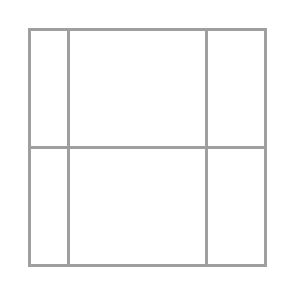
\begin{tikzpicture}[scale={1/4}]
		\plotperm{2, 4, 12, 11, 1, 3, 5, 6, 8, 7, 9, 10}
		\draw[draw=gray!75, very thick] (0.5,0.5) rectangle ++(12,12);
		\draw[draw=gray!75, very thick] (2.5,0.5) -- ++(0,12);
		\draw[draw=gray!75, very thick] (9.5,0.5) -- ++(0,12);
		\draw[draw=gray!75, very thick] (0.5,6.5) -- ++(12,0);
	\end{tikzpicture}
\caption{A $\left(\begin{smallmatrix} 0 & -1 & 1\\ 1 & 1 & 0 \end{smallmatrix}\right)$-gridding of a permutation $\pi$. As $\pi$ admits such a gridding, we write $\pi \in \gridVertThree{1,0}{1,-1}{0,1}$.}
\label{fig-m-gridding}
\end{figure}

To aid comprehension, we denote grid classes by their \emph{cell diagrams} rather than by their matrices. For example, we abbreviate $\Grid{\begin{smallmatrix} 0 & -1 & 1\\ 1 & 1 & 0 \end{smallmatrix}}$ as $\gridVertThree[{1/3}]{1,0}{1,-1}{0,1}$. Occasionally, where it is convenient, we use a cell diagram to stand for the matrix itself.

We begin the results portion of this subsection with an observation useful for providing lower bounds on the size of proper universal permutations for grid classes.

\begin{observation}
\label{obs-grid-points}
	Let $\P = \Grid{M}$ be a grid class, and let $\sigma, \pi \in \P$. If in every $M$-gridding of $\sigma$ there are $k$ points in cell $M_{i,j}$ and $\sigma \le \pi$, then in every $M$-gridding of $\pi$ there are at least $k$ points in the cell $M_{i,j}$.
\end{observation}

As one simple example where Observation~\ref{obs-grid-points} is useful, let $M = \gridHorizTwo[{1/3}]{1}{1}$ and consider the grid class $\P = \Grid{M}$. In the unique $M$-gridding of the permutation $m 12 \cdots (m-1)$, the lower cell of $M$ contains $m-1$ points, and thus any $M$-gridding of any proper $\P_m$-universal permutation must place at least $m-1$ points the lower cell of $M$. Likewise, the unique $M$-gridding of the permutation $2 \cdots m1$ places $m-1$ points in the upper cell of $M$, and thus any $M$-gridding of any proper $\P_m$-universal permutation must place at least $m-1$ points in the upper cell of $M$. Together, these observations show that any proper $\P_m$-universal permutation must have at least $2(m-1)$ points, which is nearly optimal as we will see shortly in Theorem~\ref{thm-perm-riffle}.

%%%%%%%%%%%%%%%%%%%%%%%%%%%%%%%%
%%%%%%%%%%%%%%%%%%%%%%%%%%%%%%%%
\subsection{Wedge Permutations and Riffle Shuffle Permutations}
\label{subsec-wedgle-riffle}
%%%%%%%%%%%%%%%%%%%%%%%%%%%%%%%%
%%%%%%%%%%%%%%%%%%%%%%%%%%%%%%%%

Up to symmetry, the two simplest non-trivial grid classes are $\gridVertOne[{1/3}]{-1,-1}$ and $\gridVertOne[{1/3}]{-1,1}$. In this section, we show that both classes have smallest (proper) $m$-universal permutations of size $2m-1$. To begin, let $\W = \Av(132, 312) = \gridVertOne[{1/3}]{1,-1}$ denote the class of non-empty \emph{wedge} permutations. In~\cite{bannister:superpatterns-a:}, Bannister, Cheng, Devanny, and Eppstein prove that $\W$ has smallest (proper) universal permutations of size $2m-1$, and below we provide a proof of this fact. To begin, we show that the poset of nonempty wedge permutations is isomorphic to the poset of words over a two-letter alphabet, discussed in generality in Section~\ref{sec-words}.

\begin{proposition}
\label{prop-perm-wedge-isomorphism}
Define the map $P: \{p, m\}^\ast \to \W$ recursively as follows:
\begin{enumerate}
	\item $P(\varepsilon) = 1$ is the permutation of size $1$.
	\item $P(vp) = P(v) \directsum 1$ is the direct sum of $P(v)$ with the pattern $1$.
	\item $P(vm) = P(v) \skewsum 1$ is the skew sum of $P(v)$ with the pattern $1$.
\end{enumerate}
Then $P$ is a poset isomorphism.
\end{proposition}

The map $P$ sends words of size $m$ to permutations of size $m+1$, so we omit the $0$-pattern from $\W$. Before proving Proposition~\ref{prop-perm-wedge-isomorphism}, we present a useful lemma.
\begin{lemma}
\label{lemma-perm-sum}
If $\pi$ and $\sigma$ are permutations, then
\begin{enumerate}
	\item $\pi \directsum 1 \le \sigma \directsum 1$ if and only if $\pi              \le \sigma$.
	\item $\pi \directsum 1 \le \sigma \skewsum   1$ if and only if $\pi \directsum 1 \le \sigma$.
	\item $\pi \skewsum   1 \le \sigma \directsum 1$ if and only if $\pi \skewsum   1 \le \sigma$.
	\item $\pi \skewsum   1 \le \sigma \skewsum   1$ if and only if $\pi              \le \sigma$.
\end{enumerate}
\end{lemma}

We now present the proof of Proposition~\ref{prop-perm-wedge-isomorphism}.

\newenvironment{proof-of-prop-perm-wedge-isomorphism}{%
	\medskip\noindent {\it Proof of Proposition~\ref{prop-perm-wedge-isomorphism}.\/}%
}{%
	\qed\bigskip%
}
\begin{proof-of-prop-perm-wedge-isomorphism}
	We begin by proving that if $v, w \in \{p, m\}^\ast$ with $v \le w$, then $P(v) \le P(w)$.

	Leveraging the recursive nature of the map $P$, we proceed by induction on the size of $v$. For our base case, note that if $v$ is the empty word, then $P(v) = 1$, which is contained in every non-empty permutation. Thus, assume that $v$ is a non-empty word, let $\ell$ be the final letter of $v$, and write $v = v_0 \ell$. Let $w \in \{p, m\}^\ast$ be any word with $v \le w$. As $v$ is a subsequence of $w$, we may write $w = w_0 \ell v_1$, where $v_0 \le w_0$. By induction, we have $P(v_0) \le P(w_0)$. By Lemma~\ref{lemma-perm-sum}, we have $P(v_0\ell) \le P(w_0\ell)$ no matter the value of $\ell$. Finally, as $P(w_0\ell) \le P(w_0\ell w_1)$, we have
	\[
		P(v) 
		=
		P(v_0\ell)
		\le
		P(w_0\ell)
		\le
		P(w_0\ell w_1)
		=
		P(w),
	\]
	as desired.

	For the converse, we show that if $P(v)$ and $P(w)$ are permutations with $P(v) \le P(w)$, then $v \le w$. Again, we proceed by induction on the size of $v$ and begin by noting that the permutation $P(\varepsilon) = 1$ is contained in every permutation in $\W$, and the empty word $\varepsilon$ is contained in every word in $\{p, m\}^\ast$, so the base case is satisfied.

	Let $P(v)$ and $P(w)$ be permutations with $P(v) \le P(w)$ and $\size{P(v)} \ge 2$, or equivalently, $\size{v} \ge 1$. Without loss of generality, assume that $v = v_0 p$ and $w = w_0 p m^k$ for some $k \ge 0$. Repeated applications of Lemma~\ref{lemma-perm-sum} mean that $P(v_0 p) \le P(w_0 p m^k)$ implies that $P(v_0) \le P(w_0)$. By induction we must have $v_0 \le w_0$, and thus $v_0 p \le w_0 p m^k$, completing the proof.
\end{proof-of-prop-perm-wedge-isomorphism}

One consequence of this isomorphism is that the smallest universal words constructed in Section~\ref{sec-words} translate into smallest proper universal permutations for $\W$.
\begin{corollary}
\label{cor-perm-wedge-proper}
	The smallest proper $\W_m$-universal permutations have size $2m-1$.
\end{corollary}

As $\W_m$ contains both $12 \cdots m$ and $m \cdots 21$, any $\W_m$-universal permutation must contain a length-$m$ increasing subsequence as well as a length-$m$ decreasing subsequence. As these subsequences may not intersect in more than one entry, any $\W_m$-universal permutation must have size at least $2m-1$, so no smaller $\W_m$-universal permutation exists outside $\W$.

\begin{corollary}
\label{cor-perm-wedge-improper}
	The smallest (proper) $\W_m$-universal permutations have size $2m-1$.
\end{corollary}

The other $2 \times 1$ grid class is $\R = \Av(123, 3412, 3142) = \gridVertOne{-1,-1}$, the class of \emph{riffle shuffle} permutations, so called as they are precisely those patterns that may be formed by a single riffle shuffle of a deck of $n$ cards. In~\cite{bannister:small-superpatt:}, Bannister, Devanny, and Eppstein prove that the permutation $(m+1)1(m+2)2\cdots(2m-1)(m-1) \in \R$ is $\R_m$-universal. This construction may be seen to be optimal, as we now show. Consider the layered permutation class $\P = \gridVertTwo[{1/3}]{-1,0}{0,-1}$. By Proposition~\ref{prop-layerize}, the minimum size of a $\P_m$-universal permutation is the same as the minimum size of an $m$-universal composition for the composition class $\Age(\omega^2)$, which is $2m-1$ by Proposition~\ref{prop-comp-length-2-improper}. As $\P \subseteq \R$, the smallest $\R_m$-universal permutation must have size at least $2m-1$, and thus the construction by Bannister, Devanny, and Eppstein is optimal.

\begin{theorem}
\label{thm-perm-riffle}
	Let $\R = \gridVertOne[{1/3}]{-1,-1}$. The smallest (proper) $\R_m$-universal permutations have size $2m-1$ for $m \ge 1$.
\end{theorem}

%%%%%%%%%%%%%%%%%%%%%%%%%%%%%%%%
%%%%%%%%%%%%%%%%%%%%%%%%%%%%%%%%
\subsection{\texorpdfstring{$\{123, 312\}$}{(123, 312)}-avoiding Permutations}
%%%%%%%%%%%%%%%%%%%%%%%%%%%%%%%%
%%%%%%%%%%%%%%%%%%%%%%%%%%%%%%%%

One immediate consequence of Theorem~\ref{thm-perm-riffle} is that any class of permutations that contains $\gridVertTwo[{1/3}]{-1,0}{0,-1}$ and is contained in $\gridVertOne[{1/3}]{-1,-1}$ must have smallest $m$-universal permutations of size $2m-1$. The class $\gridVertThree[{2/9}]{0,-1,0}{0,0,-1}{-1,0,0}$ meets this criteria, and thus the corollary below follows.
\begin{corollary}
\label{cor-perm-123-312-improper}
	Let $\P = \Av(123, 312) = \gridVertThree[{2/9}]{0,-1,0}{0,0,-1}{-1,0,0}$. For each $m \ge 1$, the smallest $\P_m$-universal permutations have size $2m-1$.
\end{corollary}

The size of the smallest proper $\Av(123, 312)_m$-universal permutations is slightly larger, as the following theorem shows.
\begin{theorem}
	Let $\P = \Av(123, 312) = \gridVertThree[{2/9}]{0,-1,0}{0,0,-1}{-1,0,0}$. For each $m \ge 3$, the smallest proper $\P_m$-universal permutations have size $3m-4$.
\end{theorem}
\begin{proof}
	To begin, we claim that the permutation $\pi = (\delta_{m-1} \directsum \delta_{m-1}) \skewsum \delta_{m-2}$ is $\P_m$-universal. Let $\sigma \in \P_m$. If $\sigma$ avoids $12$, then $\sigma$ is the decresing permutation of size $m$, and as $\pi$ contains $\delta_{m-2} \skewsum \delta_{m-1} = \delta_{2m-3}$ and $2m-3 \ge m$, we have that $\pi$ contains $\sigma$. Otherwise, $\sigma$ contains $12$, and we may decompose $\sigma$ as $\sigma = (\delta_a \directsum \delta_b) \skewsum \delta_c$ for nonnegative integers $a, b, c$ with $a, b \ge 1$ and $a + b + c = m$. In this case, both $a$ and $b$ must be at most $m-1$, and $c$ must be at most $m-2$, which implies that $\sigma$ is contained in $(\delta_{m-1} \directsum \delta_{m-1}) \skewsum \delta_{m-2} = \pi$.

	Let $M$ be the matrix $\gridVertThree[{2/9}]{0,-1,0}{0,0,-1}{-1,0,0}$. To establish a lower bound, we show that in any $M$-gridding of a proper $\P_m$-universal permutation, the lower-right cell must have at least $m-2$ points and both the leftmost cell and topmost cell must each have at least $m-1$ points.

	Consider the permutations $\sigma_1 = 1 \directsum \delta_{m-1}$, $\sigma_2 = \delta_{m-1} \directsum 1$, and $\sigma_3 = 12 \skewsum \delta_{m-2}$.
	\begin{enumerate}
		\item The permutation $\sigma_1 = 1 m \cdots 2$ has a unique $M$-gridding, where the $m-1$ entries $2, 3, \dots, m$ are placed in topmost cell and the entry $1$ is placed in the leftmost cell. 
		\item The permutation $\sigma_2 = (m-1)\cdots 2m$ has a unique $M$-gridding, where the entry $m$ is placed in the topmost cell and the $m-1$ entries $1, 2, \dots, (m-1)$ are placed in the leftmost cell. 
		\item The permutation $\sigma_3 = (m-1)m(m-2) \cdots 21$ has a unique gridding in $M$, where the $m-2$ entries $1, 2, \dots, (m-2)$ are placed in the lower-right cell, the entries $m-1$ and $m$ are placed in the leftmost and topmost cells, respectively.
	\end{enumerate}
	By Observation~\ref{obs-grid-points}, any $M$-gridding of any proper $\P_m$-universal permutation must contain at least $m-1$ points in the topmost cell, at least $m-1$ points in the leftmost cell, and at least $m-2$ points in the lower-left cell, and therefore must have size at least $(m-2) + (m-1) + (m-1) = 3m-4$, as desired.
\end{proof}

%%%%%%%%%%%%%%%%%%%%%%%%%%%%%%%%
%%%%%%%%%%%%%%%%%%%%%%%%%%%%%%%%
\subsection{\texorpdfstring{$\{231, 2143\}$}{231, 2143}-avoiding Permutations}
%%%%%%%%%%%%%%%%%%%%%%%%%%%%%%%%
%%%%%%%%%%%%%%%%%%%%%%%%%%%%%%%%

Let $\P = \Av(231, 2143) = \gridVertTwo[{1/3}]{1,-1}{0,1}$ be the class of $\{231, 2143\}$-avoiding permutations. In~\cite{bannister:superpatterns-a:}, Bannister, Cheng, Devanny, and Eppstein prove that there are $\P_m$-universal permutations of size $3m-4$ for $m \ge 3$. We provide a simple proof of this construction.

\begin{theorem}[Bannister, Cheng, Devanny, and Eppstein~\cite{bannister:superpatterns-a:}]
\label{thm-perm-231-2143-proper}
	For each $m \ge 3$, there is a proper $\P_m$-universal permutation of size $3m-4$.
\end{theorem}
\begin{proof}
	Let $\upsilon_3 = 51324$, and for each $m > 3$, let $\upsilon_{m+1} = 1 \skewsum (1 \directsum \upsilon_{m} \directsum 1)$. We claim that, for each $m \ge 3$, $\upsilon_m$ is (1) in $\P$ and (2) $\P_m$-universal. To begin, note that $\upsilon_3$ is in $\P$ and that for any permutation $\pi \in \P$, the permutations $1 \skewsum \pi$, $1 \directsum \pi$, and $\pi \directsum 1$ all lie in $\P$. As $\upsilon_{m+1}$ is constructed from $\upsilon_m$ using only these operations, we have that $\upsilon_m \in \P$ for all $m \ge 3$ by induction.

	To show that $\upsilon_m$ is $m$-universal for all $m \ge 3$, we begin by noting that $\upsilon_3 = 51324$ is $\P_3$-universal, meaning it contains the pattern $123$, $132$, $213$, $312$ and $321$, which we may check by hand. Given any permutation $\pi \in \P$, we may decompose $\pi$ as at least one of $\pi = 1 \directsum \pi^\ast$, $\pi = 1 \skewsum \pi^\ast$, or $\pi = \pi^\ast \directsum 1$, where $\pi^\ast \in \P_{m-1}$. As $\upsilon_m$ contains each of $1 \directsum \upsilon_{m-1}$, $1 \skewsum \upsilon_{m-1}$, and $\upsilon_{m-1} \directsum 1$, and $\upsilon_{m-1}$ contains $\pi^\ast$ necessarily by induction, we have that $\upsilon_m$ contains $\pi$, completing the proof.
\end{proof}

Moreover, Bannister, Cheng, Devanny, and Eppstein prove that, with $\Q = \Av(231, 312, 2143, 1324) = \gridHorizTwo[{1/3}]{1,0}{0,-1} \cup \gridVertTwo[{1/3}]{-1,0}{0,1}$, any $\Q_m$-universal permutation has size at least $3m-4$. As $\Q \subseteq \P$, any $\P_m$-universal permutation must have size at least $3m-4$, which together with the $\P_m$-universal permutations of size $3m-4$ of Theorem~\ref{thm-perm-231-2143-proper} are the best-possible even outside the class.
\begin{theorem}[Bannister, Cheng, Devanny, and Eppstein~\cite{bannister:superpatterns-a:}]
\label{thm-perm-231-2143-improper}
	The smallest $m$-universal permutations for $\Av(231, 2143)$ have size $3m-4$.
\end{theorem}

As a corollary, Bannister, Cheng, Devanny, and Eppstein note that any class contained in $\P$ that contains $\Q$ has smallest universal permutations of this size as well:
\begin{corollary}[Bannister, Cheng, Devanny, and Eppstein~\cite{bannister:superpatterns-a:}]
	If $\R$ is a permutation class with $\Q \subseteq \R \subseteq \P$, then the smallest $\R_m$-universal permutations have size $3m-4$.
\end{corollary}

%%%%%%%%%%%%%%%%%%%%%%%%%%%%%%
%%%%%%%%%%%%%%%%%%%%%%%%%%%%%%
\subsection{\texorpdfstring{$231$}{231}-avoiding Permutations}
%%%%%%%%%%%%%%%%%%%%%%%%%%%%%%
%%%%%%%%%%%%%%%%%%%%%%%%%%%%%%

In~\cite{knuth:the-art-of-comp:1}, Knuth shows that the permutations that may be sorted with a stack are precisely those that avoid the permutation $231$. Let $\P = \Av(231)$ denote the class of $231$-avoiding permutations. In~\cite{bannister:superpatterns-a:}, Bannister, Cheng, Devanny, and Eppstein construct $\P_m$-universal permutations of size $\floor{m^2/4} + m$ and construct, for every proper subclass of $\P$, $m$-universal permutations of size $\oO{m \log^{\oO{1}}m}$. The $\P_{10}$-universal permutation of their construction is presented in the left panel of Figure~\ref{fig-perm-231-univ}.

To present a construction of proper $\P_m$-universal permutations, we say the \emph{reverse-inverse-reverse} of a permutation $\pi$, denoted $\pi^{\rir}$, is defined as $\pi^{\rir} = ((\pi^{r})^{-1})^{r}$, where $\pi^r$ is the permutation formed by reversing $\pi$, and $\pi^{-1}$ is the function inverse of $\pi$. Pictorially, a plot of $\pi^{\rir}$ may be obtained by reflecting the plot of $\pi$ across the line $y = -x$. The reverse and inverse symmetries preserve containment, so the reverse-inverse-reverse symmetry does as well, meaning that $\sigma \le \pi$ if and only if $\sigma^{\rir} \le \pi^{\rir}$. As $231 = 231^{\rir}$, the class $\P$ is closed under the reverse-inverse-reverse symmetry, and thus $\pi$ is $\P_m$-universal if and only if $\pi^{\rir}$ is.

\begin{proposition}
\label{prop-perm-231-proper}
Let $\Pi_0 = \varepsilon$, and for $m \ge 1$, define
\[
	\Pi_m
	=
	\left(1 \skewsum \Pi_{m-1}^{\rir}\right) \directsum \Pi_{\floor{m/2}}.
\]
Then $\Pi_{m}$ is a proper $\P_m$-universal permutation for all $m$.
\end{proposition}

\begin{figure}
\captionsetup{justification=centering}
	\begin{tikzpicture}[scale={6/35}]
		\draw (0.25,0.35) rectangle ++(35.5, 35.5);
		\plotperm{34,23,14,7,2,1,33,22,13,6,3,32,21,12,5,4,31,20,11,8,30,19,10,9,29,18,15,28,17,16,27,24,26,25,35}

		\begin{scope}[shift={(40,0)}]
			\draw (0.25,0.35) rectangle ++(35.5, 35.5);
			\plotperm{26,1,5,3,2,4,25,19,7,6,8,18,14,9,13,11,10,12,16,15,17,20,24,22,21,23,32,27,31,29,28,30,34,33,35}
		\end{scope}
	\end{tikzpicture}
\caption{On the left, the $\P_{10}$-universal permutation of size $35$ of Bannister, Chung, Devanny, and Eppstein's construction~\cite{bannister:superpatterns-a:}. On the right, the proper $\P_8$-universal permutation $\Pi_{8}$ of size $35$.}
\label{fig-perm-231-univ}
\end{figure}

\begin{proof}
	Before showing that $\Pi_{m}$ is $\P_m$-universal for each $m$, we show that each $\P_m$ lies in $\P$ by a brief inductive arguemnt. The permutation $\Pi_0 = \varepsilon$ lies in every class of permutations, so our base case is satisfied. In addition to being closed under the reverse-inverse-reverse symmetry, the class $\P$ is closed under prepending a new largest element and under direct sums, ie. if $\pi, \sigma \in \P$, then both $1 \skewsum \pi$ and $\pi \directsum \sigma$ lie in $\P$. Thus, by induction, $\Pi_{m} = (1 \skewsum \Pi_{m-1}^{\rir}) \directsum \Pi_{\floor{m/2}} \in \P$ for all $m$.

	To show that $\Pi_{m}$ is $\P_m$-universal for all $m$, we again proceed by induction on $m$. The permutation $\Pi_0 = \varepsilon$ is clearly $0$-universal for every class, so assume that $\Pi_{m'}$ is $m'$-universal for $\P$ for all $m' < m$.

	Let $\pi \in \P_m$. If $\pi$ is sum-indecomposable, then $\pi = 1 \skewsum \tau$ for some $\tau \in \P_{m-1}$. As $\Pi_{m-1}$ is $\P_{m-1}$-universal, $\Pi^{\rir}_{m-1}$ is as well. Thus, as $\Pi_m$ contains $1 \skewsum \Pi^{\rir}_{m-1}$ and $\pi = 1 \skewsum \sigma$ for $\sigma \in \P_{m-1}$, we have that $\pi \le \Pi_m$. 
	
	Otherwise, we may write $\pi = \pi_{1} \directsum \pi_{2}$, where $\pi_{2}$ is a non-empty sum-indecomposable permutation, and we complete our analysis in two cases: when $\size{\pi_{2}} \le \floor{m/2}$ and when $\size{\pi_{2}} \ge \floor{m/2} + 1$. In the first case, assume that $\size{\pi_{2}} \le \floor{m/2}$. As $\size{\pi_{1}} \le m-1$, we have that $\pi_{1}$ embeds into $\Pi_{m-1}^{\rir}$, and as $\size{\pi_{2}} \le \floor{m/2}$, we have that $\pi_{2}$ embeds into $\Pi_{\floor{m/2}}$. Since $\Pi_{m}$ contains $\Pi_{m-1}^{\rir} \directsum \Pi_{\floor{m/2}}$, we may conclude that $\pi = \pi_{1} \directsum \pi_{2} \le \Pi_{m}$. In the second case, assume that $\size{\pi_{2}} \ge \floor{m/2}+1$, and thus $\size{\pi_{1}} \le \ceil{m/2}-1$. We claim that $\pi$ embeds into $\Pi_{m-1}^{\rir} = \Pi_{k-1}^{\rir} \directsum (1 \skewsum \Pi_{m-2})$. As $\pi_{2}$ is sum-indecomposable, we may write $\pi_{2} = 1 \skewsum \tau$ for some $\tau$ with $\size{\tau} \le m-2$. Thus we have $\pi = \pi_{1} \directsum (1 \skewsum \tau)$, where $\size{\pi_{1}} \le k-1$ and $\size{\tau} \le 2k-2$, and so by induction, $\pi$ embeds into $\Pi_{k-1}^{\rir} \directsum (1 \skewsum \Pi_{2k-2}) = \Pi_{2k-1}^{\rir}$, completing the proof.
\end{proof}

\begin{corollary}
\label{cor-231-ub-formula}
The sequence $\size{\Pi_{m}} = p(m)$ is given by $p(0) = 0$ and, for $m \ge 1$,
\[
	p(m) 
	= 
	p(m-1) + p\left(\floor{m/2}\right) + 1,
\]
and thus the smallest proper $\P_m$-universal permutations have size at most $p(m)$.
\end{corollary}

The proper $\P_m$-universal permutations constructed in Proposition~\ref{prop-perm-231-proper} are much larger than the $\P_m$-universal permutations of size $\floor{m^2/4} + m$ constructed by Bannister, Cheng, Devanny, and Eppstein in~\cite{bannister:superpatterns-a:}, as the next result shows.

\begin{theorem}[Knuth~\cite{knuth:an-almost-linear:}]
\label{thm-almost-linear}
Let $a(1) = 1$ and $a(n) = a(n-1) + a(\floor{n/2})$ for $n \ge 2$. Then $a(n)$ grows faster than any polynomial. That is, for any power $k$, there is some $N_k$ such that for all $n \ge N_k$ we have $a(n) > n^k$.
\end{theorem}

Before presenting the proof of Theorem~\ref{thm-almost-linear}, note that $s(n) \ge a(n)$, and thus $s$ grows faster than any polynomial.

\newenvironment{proof-of-thm-almost-linear}{%
	\medskip\noindent {\it Proof of Proposition~\ref{thm-almost-linear}.\/}%
}{%
	\qed\bigskip%
}
\begin{proof-of-thm-almost-linear}
	Fix $k$. We aim to show that for sufficiently large $n$, we have $a(n) > n^k$. Let $N$ be such that 
	\[
		2^{k+1} + 1 \ge \left(2 + \frac{1}{N}\right)^{k+1}
	\]
	and let
	\[
		c 
		=
		\min\left\{\frac{a(n)}{n^{k+1}} \st N \le n \le 2N\right\}.
	\]
	We claim that for all $n \ge N$, we have $a(n) \ge cn^{k+1}$. For $N \le n \le 2N$, this is clear as $c \le a(n)/n^{k+1}$. If $n > 2N$, induction shows that
	\begin{align*}
		a(n)
			&= a(n-1) + a(\floor{n/2}) \\
			&\ge c\cdot(n-1)^{k+1} + c\cdot\floor{n/2}^{k+1} \\
			&\ge c\left((n-1)^{k+1} + \left(\frac{n-1}{2}\right)^{k+1}\right) \\
			% &=   c\left( 1 + 1/2^{k+1}             \right)     (n-1)^{k+1} \\
			&=   c\left( \frac{2^{k+1}+1}{2^{k+1}} \right)     (n-1)^{k+1} \\
			&\ge c\left( \frac{2+\frac{1}{N}}{2} \right)^{k+1} (n-1)^{k+1} \\
			&=   c\left( 1+\frac{1}{2N}          \right)^{k+1} (n-1)^{k+1} \\
			&\ge c\left( 1+\frac{1}{n-1}         \right)^{k+1} (n-1)^{k+1} \\
			&=   c n^{k+1}.
	\end{align*}
	
	To conclude, choose $N_k$ such that $N_k \ge N$ and $N_k \ge 1/c$ (so that $cn \ge c N_k \ge 1$), and the proof is complete.
\end{proof-of-thm-almost-linear}

%%%%%%%%%%%%%%%%%%%%%%%%%%%%%%%%
%%%%%%%%%%%%%%%%%%%%%%%%%%%%%%%%
\subsection{\texorpdfstring{$321$}{321}-avoiding Permutations}
%%%%%%%%%%%%%%%%%%%%%%%%%%%%%%%%
%%%%%%%%%%%%%%%%%%%%%%%%%%%%%%%%

Let $\S$ be the class of $321$-avoiding permutations. Equivalently, $\S$ is the class of permutations that may be partitioned into two increasing subsequences. In~\cite{bannister:small-superpatt:}, Bannister, Devanny, and Eppstein construct $\S_m$-universal permutations of size $22m^{3/2} + \oTheta{m}$.

In~\cite{Atminas:Universal-graph:}, Atminas, Kitaev, Lozin, and Valyuzhenich construct a proper $\S_m$-universal permutation of size $m^2$. The corresponding permutation graph is thus a proper $\g(\S)_m$-universal graph, where in this case $\g(\S)$ is the class of bipartite permutation graphs. This corresponding $\g(\S)_m$-universal permutation graph is in fact equal to the size-$m^2$ graph that Lozin and Rudolf construct in \cite{lozin:minimal-univers:}. The question of whether $\S$ admits sub-quadratic sized proper universal permutations remains open, but evidence points towards ``no''. In~\cite{alecu:critical-properties:}, Alecu, Lozin, and Malyshev prove that any proper $m$-universal graph for the class of bipartite permutation graphs must have size $\oOmega{m^\alpha}$ for all $\alpha < 2$, implying that any proper $\S_m$-universal permutation must have size $\oOmega{m^\alpha}$ for all $\alpha < 2$. They conjecture that the smallest $m$-universal graphs for the class of bipartite permutation graphs have size $\oOmega{m^2}$, which would imply that the smallest proper $\S_m$-universal permutations have size $\oTheta{m^2}$.

%%%%%%%%%%%%%%%%
%%%%%%%%%%%%%%%%
%%%%%%%%%%%%%%%%
%%%%%%%%%%%%%%%%
\subsection{Subclasses of \texorpdfstring{$\Av(321)$}{Av(321)}: Truncated Staircases}
%%%%%%%%%%%%%%%%
%%%%%%%%%%%%%%%%
%%%%%%%%%%%%%%%%
%%%%%%%%%%%%%%%%

The class $\Av(321)$ may be represented as the grid class of an infinite matrix. First shown by Albert, Atkinson, Brignall, Ru\v{s}kuc, Smith, and West~\cite{albert:growth-rates-fo:}, we have
\[
	\Av(321)
	=
	\begin{tikzpicture}[grids]

		\foreach \x in {0, 1, 2, 3, 4} {
			\draw [thin, gray] (\x,0) -- ++(0,3.9);
		}

		\foreach \y in {0, 1, 2, 3} {
			\draw [thin, gray] (0,\y) -- ++(4.9,0);
		}

		\draw (0,0) rectangle ++(1,1);
		\draw[ultra thick, shorten <=4pt, shorten >=4pt] (0,0) -- ++(1,1);
		\draw (1,0) rectangle ++(1,1);
		\draw[ultra thick, shorten <=4pt, shorten >=4pt] (1,0) -- ++(1,1);
		\draw (1,1) rectangle ++(1,1);
		\draw[ultra thick, shorten <=4pt, shorten >=4pt] (1,1) -- ++(1,1);
		\draw (2,1) rectangle ++(1,1);
		\draw[ultra thick, shorten <=4pt, shorten >=4pt] (2,1) -- ++(1,1);
		\draw (2,2) rectangle ++(1,1);
		\draw[ultra thick, shorten <=4pt, shorten >=4pt] (2,2) -- ++(1,1);
		\draw (3,2) rectangle ++(1,1);
		\draw[ultra thick, shorten <=4pt, shorten >=4pt] (3,2) -- ++(1,1);
		\foreach \d in {0.25, 0.50, 0.75} {
			\filldraw[black] ({3+\d}, {3+\d}) circle [radius=0.03cm];
			\filldraw[black] ({4+\d}, {3+\d}) circle [radius=0.03cm];
		}
	\end{tikzpicture}
\]

The figure on the right is known as the infinite \emph{positive staircase}. One natural family of subclasses of $\Av(321)$ are the finite positive staircases. Let $\S^k$ be the positive staircase consisting of the first $k$ nonempty cells of the infinite staircase, e.g, $\S^1 = \gridCell[{1/3}]{1}$, $\S^2 = \gridHorizOne[{1/3}]{1,1}$, $\S^3 = \gridHorizTwo[{1/3}]{1,1}{0,1}$, and so on.

Then, as 
\[
	\S^1
	\subseteq
	\S^2
	\subseteq
	\S^3
	\subseteq
	\cdots
	\subseteq
	\S,
\]
we have
\[
	\u_{\S^1}(m)
	\le
	\u_{\S^2}(m)
	\le
	\u_{\S^3}(m)
	\le
	\cdots
	\le
	\u_{\S}(m).
\]

For all $m$, every permutation in $\S_m$ may be gridded using the first $\ceil{(m+1)/2}$ cells of the infinite positive, and there is some permutation in $\S_m$ that cannot be gridded using $\ceil{(m-1)/2}$ cells. Thus, any proper $\S_m$-universal permutation may not use fewer than the first $\ceil{(m+1)/2}$ cells, and computation suggests that among all smallest proper $\S_m$-universal permutations, there is at least one that may itself be gridded in $\ceil{(m+1)/2}$ cells. 
\begin{conjecture}
\label{conj-no-more-cells}
For all $m \ge 0$, there is a smallest proper $\S_m$-universal permutation that lies in $\S^{\ceil{(m+1)/2}}$.
\end{conjecture}

We now demonstrate, through Observation~\ref{obs-grid-points}, a lower bound on the size of proper $\S^{k}_m$-universal permutations. For $k \ge 2$, let $M$ be the matrix corresponding to the the finite positive staircase with $k$ nonempty cells. The permutation $\pi = 21 43 \cdots (2k-2)(2k-3)$ has a unique $M$-gridding, placing one point in each of the first and last cells and two points in every other cell. Consider some entry $\pi(i)$ of $\pi$ that is placed in the cell $C$ in the unique $M$-gridding of $\pi$. Replacing the entry $\pi(i)$ of $\pi$ with a contiguous increasing sequence of entries of size $m-2k+3$ and yields a permutation of size $m$ that has a unique $M$-gridding, placing $m-2k+3$ points in the cell $C$ if $C$ is the first or last cell of $M$ or $m-2k+4$ points in the cell $C$ otherwise. 

Thus for $m \ge 2k-2$, any $M$-gridding of a proper $\S^k_m$-universal permutation must have at least $m-2k+3$ points in its first and last cells, and $m-2k+4$ points in each of its other $k-2$ cells. This shows that any proper $\S^k_m$-universal permutation must have size at least $2(m-2k+3) + (k-2)(m-2k+4) = km - 2(k-1)^2$.

\begin{proposition}
\label{prop-cells-proper-lower}
	For $m \ge 2k-2$, any proper $\S^k_m$-universal permutation has size at least $km - 2(k-1)^2$.
\end{proposition}

Using Conjecture~\ref{conj-no-more-cells} and Proposition~\ref{prop-cells-proper-lower}, we have the conjollary\footnote{A \emph{conjollary} is a corollary that follows from a conjecture.} below.
\begin{conjollary}
	For all $m \ge 4$, any proper $\S_m$-universal permutation must have size at least $m^2/8$.
\end{conjollary}
\begin{proof}
	By Conjecture~\ref{conj-no-more-cells}, we have that the size of the smallest proper $\S_m$-universal permutations and the size of the smallest proper $\S^k_m$-universal permutations are the same for all $k \le (m+2)/2$. By Proposition~\ref{prop-cells-proper-lower}, every proper $\S^k_m$ universal permutation has size at least $km - 2(k-1)^2$, and thus
	\begin{align*}
		\u_{\S}^p(m) 
			&\ge \max\{mk - 2(k-1)^2 \st k \le (m+2)/2\} \\
			&\ge m \floor{\frac{m}{4}+1} - 2 \floor{\frac{m}{4}}^2 \\
			&> \frac{m^2}{8},
	\end{align*}
	as desired.
\end{proof}

%%%%%%%%%%%%%%%%%%%%%%%%%%%%%%%%
%%%%%%%%%%%%%%%%%%%%%%%%%%%%%%%%
\subsection{Skew riffle Permutations}
%%%%%%%%%%%%%%%%%%%%%%%%%%%%%%%%
%%%%%%%%%%%%%%%%%%%%%%%%%%%%%%%%

We say that $\pi$ is a \emph{skew riffle} permutation if it is the sum of riffle and antiriffle permutations. Let $\SR$ be the class of skew riffle permutations:
\[
	\P
	=
	\bigdirectsum 
	\left(
		\gridVertTwoDisplay{1}{1}
		\cup 
		\gridVertOneDisplay{1,1}
	\right).
\]

In~\cite{bannister:small-superpatt:}, Bannister, Devanny, and Eppstein construct $\P_m$-universal permutations of size $16m \log m + \oTheta{m}$. Let $\R = \gridVertTwo[{1/3}]{1}{1} \cup \gridVertOne[{1/3}]{1,1}$. The permutation 
\[
	\pi_m 
	= 
	1 3 5 \cdots (2m-1) 2 (2m) 4 (2m+1) 6 \cdots (3m-3) (2m-2) (3m-2)
\]
of size $3m-2$ is $\R_m$-universal, as the lowest $2m-1$ values form the permutation $1 3 5 \cdots (2m-1) 2 4 6 \cdots (2m-2)$, which is $m$-universal for $\gridVertTwo[{1/3}]{1}{1}$, and the rightmost $2m-1$ values form the permutation $m 1 (m+1) 2 \cdots (m-1) (2m-1)$, which is $m$-universal for $\gridVertOne[{1/3}]{1,1}$. In the language of Proposition~\ref{prop-an-upper-bound}, $\comp(\R)$ is the class of all compositions, and the recursively-defined composition $w_m = w_{\floor{(m-1)/2}} m w_{\ceil{(m-1)/2}}$ (with $w_0 = \varepsilon$) of length $m$ and size $\ell(m)$ is $m$-universal. Thus the permutation $\tau_m = \directsum_{i = 1}^{m} \pi_{w_m(i)}$ is $\R_m$-universal and has size at most $3\ell(m) \sim 3m \log_2 m$. For example, Figure~\ref{fig-perm-construction} shows the plots of $\pi_4$ and $\tau_3$.

\begin{figure}
\captionsetup{justification=centering}
	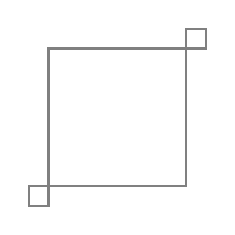
\begin{tikzpicture}[scale=0.25]
		\plotpermborder{1,3,5,7,2,8,4,9,6,10}
		\begin{scope}[shift={(12,0.5)}]
			\draw[thick, gray] (0.5,0.5) rectangle ++(1,1);
			\draw[thick, gray] (1.5,1.5) rectangle ++(7,7);
			\draw[thick, gray] (8.5,8.5) rectangle ++(1,1);
			\plotpermborder{1,2,4,6,3,7,5,8,9}
		\end{scope}
	\end{tikzpicture}
\caption{On the left, the permutation $\pi_4$, which is $4$-universal for $\gridVertTwo[{1/3}]{1}{1} \cup \gridVertOne[{1/3}]{1,1}$. On the right, the $\P_3$-universal permutation $\tau_3$ with its summands $\pi_1$, $\pi_3$, and $\pi_1$ outlined.}
\label{fig-perm-construction}
\end{figure}

%%%%%%%%%%%%%%%%%%%%%%%%%%%%%%%%
%%%%%%%%%%%%%%%%%%%%%%%%%%%%%%%%
\section{Concluding Remarks}
%%%%%%%%%%%%%%%%%%%%%%%%%%%%%%%%
%%%%%%%%%%%%%%%%%%%%%%%%%%%%%%%%

Unlike in the context of graphs, there is no clear guess about the ``optimal'' size of an $m$-universal permutation for a class based on the number of $m$-patterns in the class. Both the class of wedge permutations and the class of layered permutations contain precisely $2^{m-1}$ patterns of size $m$, but their smallest (proper) universal permutations have sizes $\ell(m) \sim m \log_2 m$ and $2m-1$, respectively. One immediately desirable characterization would be of those maximal permutation classes that admit linear-size universal permutations. 
\begin{question}
	What are the maximal permutations classes that admits linear-size universal permutations?
\end{question}
